% Training-Adaptive Data Selection with a Reliability Gate (TAG).
% Draft root file for Information Fusion review.
\documentclass[sigconf,anonymous,review]{acmart}

% ---- ACM boilerplate (vestigial, see MIGRATION NOTE) ----------------
\settopmatter{printacmref=false}
\setcopyright{none}
\renewcommand\footnotetextcopyrightpermission[1]{}
\pagestyle{plain}
\acmConference[CIKM '26]{The 35th ACM International Conference on
  Information and Knowledge Management}{November 7--11, 2026}{Rome, Italy}

% Allow large two-column floats to occupy the top of a page.
\setcounter{topnumber}{3}
\setcounter{dbltopnumber}{2}
\renewcommand{\topfraction}{0.90}
\renewcommand{\dbltopfraction}{0.95}
\renewcommand{\textfraction}{0.05}
\renewcommand{\floatpagefraction}{0.80}
\renewcommand{\dblfloatpagefraction}{0.80}

% ---- Packages -------------------------------------------------------
% De-duplicated (2026-08-13): xcolor was loaded three times with
% inconsistent options (plain, then twice with [table]) — an option
% clash on a clean compile; now loaded once as [table]{xcolor}, which
% also covers colortbl. Duplicate amsmath/amsthm/booktabs/array/
% tabularx and a duplicate \usetikzlibrary call dropped.
\usepackage{amsthm}
\makeatletter
\def\@@proof[#1]{\par\pushQED{\qed}%
  \normalfont \topsep0pt \partopsep0pt
  \trivlist\item[\hskip\labelsep\itshape#1\@addpunct{.}]\ignorespaces}
\makeatother
\usepackage{amsmath,amssymb}
\usepackage{mathtools}
\usepackage{booktabs}
\usepackage{enumitem}
\usepackage{algorithm}
\usepackage{algorithmic}
\usepackage{tikz}
\usetikzlibrary{arrows.meta,positioning}
\usepackage[normalem]{ulem}
\usepackage[table]{xcolor}
\usepackage{threeparttable}
\usepackage{kotex}
\usepackage{multirow}
\usepackage{pifont}
\newcommand{\cmark}{\ding{51}}
\newcommand{\xmark}{\ding{55}}
\usepackage{graphicx}
\usepackage{pgfplots}
\pgfplotsset{compat=1.18}
\usepackage{array}
\usepackage{tabularx}
\usepackage{capt-of} % for \captionof{table}

\newcolumntype{Y}{>{\raggedright\arraybackslash}X}

% ---- Theorem environments -------------------------------------------
\newtheorem{theorem}{Theorem}
\newtheorem{corollary}{Corollary}
\newtheorem{lemma}{Lemma}
\newtheorem{proposition}{Proposition}
\usepackage{float}
\usepackage{placeins}


% ---- Project macros -------------------------------------------------
% \STATUS{...} marks a value to be filled from final experiments.
\newcommand{\STATUS}[1]{\textcolor{red}{[#1]}}
% \TODO{...} marks an in-progress item.
\newcommand{\TODO}[1]{\textcolor{red}{[TODO: #1]}}

% =====================================================================
\begin{document}

\title{Training-Adaptive Data Selection with a Reliability Gate:
       Multi-View Fusion for Low-Quality Instruction Data}

\author{Anonymous Author(s)}

\begin{abstract}
High-quality instruction data is essential for effective instruction
tuning, but quality is inherently multi-dimensional: a useful
training set must contain not only reliable instruction--response
pairs, but also examples that directly benefit the model at its
current stage of learning. The latter cannot be determined once and
for all before training, because an example's usefulness changes as
the model is updated. Dynamic selection---re-evaluating candidates
against the evolving model---is therefore critical to constructing
an effective instruction-tuning set. This requirement becomes more
challenging in real, low-quality instruction pools, where mismatched
pairs, truncated responses, and subtly wrong answers are common:
difficulty--uncertainty signals can actively \emph{prefer} such
corruption because broken samples appear hard. From this perspective,
we propose \textsc{TAG} (\textbf{T}raining-\textbf{A}daptive data
selection with a reliability \textbf{G}ate), a three-view selection
architecture that combines a static reliability gate with two
dynamic utility signals. A static \emph{Reliability} view assigns
each sample a continuous weight \(G_i\in[0,1]\) before training,
using a counterfactual likelihood contrast --- how much the true
instruction improves the response's likelihood over an unrelated one.
The weight is zero-anchored, calibrated on a clean reference pool,
and cached at no per-refresh cost. Two
dynamic views guide training-adaptive selection: a
difficulty--uncertainty carrier \(\mathcal{R}_i^{(t)}\), and a
state-conditioned representation anchor. At each refresh, the anchor
is the principal direction of within-sequence representation
displacements on a probe subset at the current checkpoint; each
candidate's normalized projection onto this anchor provides a bounded
modulation of the carrier. A local analysis characterizes the
stability of the recomputed principal direction. The fused
score is simply \(s_i^{(t)} = G_i \cdot \mathcal{R}_i^{(t)}
\bigl(1+\lambda\,\widetilde a_i^{(t)}\bigr)\). This
multiplicative form continuously attenuates candidates according to
estimated reliability, while the dynamic terms keep selection
adaptive to the evolving model state. On
instruction pools with typed, manifest-verified corruptions
(mismatched, noisy, truncated, wrong-answer, duplicated),
\STATUS{detection and end-to-end SFT results pending: Dirty@\(K\)/AUPRC
and seed-paired benchmark comparisons vs.\ entropy-, perplexity-,
and IFD-based selection}; in prior same-protocol comparisons the
underlying training-adaptive selector already outperformed strong
static and dynamic baselines while reducing
selection-and-tuning cost by 33\% relative to a Reward+PPO selector.
\textsc{TAG} requires no external judges, reward models, or
PPO-style selector training.
\end{abstract}


\keywords{Multi-view fusion, Low-quality data, Instruction tuning,
Training-adaptive data selection, Reliability, Representation anchors,
Hidden-state geometry, Foundation models}

\maketitle

% ---- Body -----------------------------------------------------------
%==================================================================
%  Section 1: Introduction.
%=====================================================================
\section{Introduction}
\label{sec:intro}
Supervised fine-tuning (SFT) is a central stage in modern open-weight
LLM post-training recipes such as Llama, Qwen, and
Mistral~\cite{dubey2024llama3,qwen2025technical,jiang2023mistral}.
Although these recipes differ in scale, supervision, and alignment
objectives, they share a common dependency: the SFT data determines
the first task-facing adaptation of the base model and shapes the
model state on which later preference optimization or reinforcement
learning operates. High-quality instruction data is therefore a
primary determinant of effective adaptation, making its selection a
practical bottleneck for efficient and reliable post-training. Yet
quality is not a single scalar: a candidate must both provide
credible supervision and offer learning value to the model at its
current training state.

\paragraph{Two axes of instruction-data quality.}
These requirements define two related but non-substitutable axes.
\emph{Reliability} asks whether a response provides credible
supervision for its instruction, whereas \emph{usefulness} asks
whether learning from that credible pair benefits the current model.
A reliable example may already be mastered or redundant, and its
learning value may change as other capabilities are acquired.
Reliability is therefore a pair-level admissibility question that can
be assessed once before fine-tuning; usefulness is model-dependent
and must be re-evaluated as training progresses. This distinction
implies an ordered selection process: first screen or suppress
unreliable supervision, then dynamically rank the remaining
candidates by their current learning value.

\paragraph{From static scoring to dynamic usefulness.}
A one-time assessment is appropriate for reliability but insufficient
for model-dependent usefulness. Most instruction-data selection
methods score and rank candidates once before fine-tuning.
Quality-based methods use external judges or learned quality
estimators; target-conditioned methods estimate influence relative
to a validation or few-shot target set; and representation-based
methods project candidate activations onto target-derived hidden-state
directions. A more recent line of dynamic data selection instead
re-estimates candidate utility as the model state changes during
training~\cite{kung2023activeit, sun2025dots}. This line highlights a
key fact: an example's usefulness is not a static property of the
data alone, but depends on the current model, training stage, and
optimisation regime. Once unreliable supervision has been screened,
dynamic selection is therefore the critical mechanism for identifying
which remaining examples offer the greatest learning value at the
current stage. We focus on supervised instruction tuning, where
candidates are instruction--response pairs and no rollout group,
verifier reward, or target validation set is assumed.

\paragraph{Three gaps in reliable training-adaptive selection.}
Despite this progress, three gaps remain. First, existing dynamic
pipelines generally rank the full candidate pool without first
establishing whether its supervision is trustworthy. A static
reliability gate serves an orthogonal role: it asks whether a pair is
admissible before the dynamic selector asks how useful that pair is
to the current model. It is not another model-dependent difficulty or
uncertainty metric, but a new pre-selection stage that establishes a
credible candidate pool for dynamic ranking.

Second, within that credible pool, structural hidden-state
selection~\cite{nait2026} and dynamic
selection~\cite{kung2023activeit, sun2025dots, dataagent}
have largely evolved separately. Hidden-state directions are
typically fixed before training~\cite{nait2026}, while dynamic
rankings rely on scalar utilities such as difficulty or uncertainty.
Consequently, a selector can track scalar utility without also using
a representation-geometric signal recomputed from the current model
state.

Third, scalar utilities can be sensitive in heterogeneous multi-task
instruction pools. In composite-reward selectors, the variance-ratio
weight that mixes difficulty and uncertainty can reflect between-task
scale differences as well as within-task informativeness. This
confounding calls for a role-separated fusion in which the
representation signal enters as an explicitly bounded, interpretable,
and independently ablatable modulation.

The absence of the first stage is especially consequential in
low-quality instruction pools, where mismatched pairs, truncated
responses, and subtly wrong answers are
common~\cite{honovich2023unnatural,alpagasus}. The dynamic
utility signals above presuppose that the pair itself can be trusted,
yet difficulty- or uncertainty-driven selection can actively
\emph{prefer} corruption because it can raise loss and entropy in the
same direction as a genuinely hard clean pair. This is the
instruction-tuning analogue of the hard-versus-mislabeled ambiguity
long documented for
classification~\cite{pleiss2020aum,swayamdipta2020cartography,rholoss2022}:
hardness scores conflate ``hard because informative'' with ``hard
because broken.'' A reliability gate addresses this prior question
on an orthogonal axis; it does not replace dynamic selection, but
makes dynamic selection meaningful by restricting utility
comparisons to examples with credible supervision.

\paragraph{Our approach: reliability-gated, state-conditioned
selection.}
We propose \textsc{TAG} (\textbf{T}raining-\textbf{A}daptive data
selection with a reliability \textbf{G}ate). \textsc{TAG} brings the
two quality axes together in a three-view selector: a static
reliability estimate and two training-adaptive utility signals. The
gate assigns each instruction--response pair a continuous reliability
weight \(G_i\in[0,1]\) at the base checkpoint and caches it. At each
refresh step~\(t\), the current model supplies a
difficulty--uncertainty reward \(\mathcal R_i^{(t)}\) and a
state-conditioned representation-anchor signal, giving the score
\begin{equation}
s_i^{(t)}
=
\underbrace{G_i}_{\substack{\text{reliability gate}\\ \text{(static, once)}}}
\;\cdot\;
\underbrace{\mathcal{R}_i^{(t)}}_{\text{dynamic reward}}
\;\cdot\;
\underbrace{\bigl(1+\lambda\,\widetilde a_i^{(t)}\bigr)}_{\text{bounded anchor modulation}}.
\label{eq:tag-score}
\end{equation}
At each refresh, \(\widetilde a_i^{(t)}\in[0,1]\) is the
candidate's normalized projection onto per-layer principal
representation-displacement directions extracted from a current
probe subset. We use these sign-oriented directions as a
state-conditioned representation anchor. The parameter
\(\lambda\ge0\) controls the modulation strength, so the anchor
factor is confined to \([1,1+\lambda]\) and can be ablated by
setting \(\lambda=0\). The multiplicative gate is not a hard binary
filter: for \(G_i>0\) it continuously attenuates each candidate
according to its estimated reliability, while its zero anchor makes
\(G_i=0\) an exact veto that no amount of dynamic utility can
compensate; the two dynamic terms determine a credible pair's
usefulness to the evolving model.

\paragraph{Design rationale.}
Three choices support this construction. First, the reliability gate
acts as a detector of instruction--response dependency rather than a
classifier of corruption types: an instruction-side counterfactual
asks how strongly the response depends on its paired instruction and
maps that evidence to a continuous reliability gate. Second,
because the representation anchor is recomputed during training, its
local directional stability matters. Under optimiser-scale covariance
drift and positive cross-time spectral separation, a Davis--Kahan
analysis gives a conditional \(O(\eta_t)\) one-step bound on the
sign-oriented principal direction. This does not guarantee stability
of candidate projections or of the full ranking; the bounded factor
instead limits the anchor's direct modulation of the reward. Third,
the dynamic score is
analytically motivated: a total-variance decomposition shows that a
difficulty--uncertainty mixture can entangle within-task
informativeness with between-task scale differences, motivating the
addition of a distinct and explicitly bounded representation signal.

\paragraph{Contributions.}
We make four contributions:
\begin{itemize}
  \item We introduce \textsc{TAG}, a training-adaptive selection
  framework that combines a continuous, static reliability gate
  with dynamic estimates of model-dependent usefulness.
  \item We develop an instruction-side counterfactual detector that
  aggregates response-level, span-level, and completeness evidence
  into a reliability gate \(G_i\in[0,1]\), computed once and cached.
  \item We provide analytical support for the dynamic selector: a
  total-variance decomposition motivates the role-separated reward
  design, and a conditional local stability result characterizes the
  recomputed principal direction, whose normalized candidate projection
  provides a bounded modulation of that reward.
  \item We evaluate \textsc{TAG} on instruction pools with typed,
  manifest-verified corruptions (mismatched, noisy, truncated,
  wrong-answer, and duplicated), measuring both corruption detection
  (Dirty@\(K\)/AUPRC) and end-to-end SFT quality against static and
  dynamic selection baselines; \STATUS{results pending}.
\end{itemize}





\section{Related Work}
\label{sec:related}

\paragraph{Multi-view quality for instruction data.}
Instruction-data quality is inherently multi-faceted. Huang
et al.~\cite{huang2024ivm} formalize instruction mining through three
views---diversity, complexity, and accuracy---and fuse LoRA-space
coverage, uncertainty-based complexity, and reward-model accuracy to
select a compact tuning subset. Closely related instruction-selection
methods likewise combine several notions of quality: DEITA
integrates complexity, quality, and diversity~\cite{deita}; MoDS
balances quality, coverage, and necessity~\cite{mods}; SelectIT uses
uncertainty-aware self-reflection~\cite{selectit}; and IFD/Q2Q ranks
examples by model-derived instruction-following
difficulty~\cite{q2q}. These works establish that no single scalar
fully describes useful instruction data. Their views, however, are
typically evaluated and fused before fine-tuning. Our setting adds a
temporal distinction: pair reliability is assessed once, whereas the
usefulness of a reliable pair is refreshed as the model learns.

\paragraph{Quality filtering under unreliable supervision.}
Real instruction pools contain noisy, mismatched, incomplete, or
otherwise unreliable supervision. Quality-filtering methods address
this problem using learned estimators or stronger LLM
judges~\cite{alpagasus,cpqs2026}, while reward-model accuracy in
multi-view instruction mining provides an explicit correctness
signal~\cite{huang2024ivm}. More broadly, trusted multi-view learning
studies how evidence sources with unequal or conflicting reliability
should influence fusion~\cite{tmc2021,rcml2024}. TAG brings this
reliability-aware perspective to instruction-data selection. Its
static view is an instruction--response dependency detector whose
continuous gate attenuates questionable supervision before two
model-dependent utility signals are combined. This role differs from
both a global quality ranking and a corruption-type classifier: the
gate estimates the credibility of the pair, while dynamic selection
decides how useful that pair is at the current training stage.

\paragraph{Static target-conditioned and representation-based
selection.}
Other selectors define usefulness relative to a target distribution
or internal model geometry. DSIR uses importance resampling for
language-model data selection~\cite{dsir}; LESS scores candidates by
gradient similarity to a validation or few-shot target
set~\cite{less}; and Approx-LESS improves the scalability of this
influence calculation~\cite{approxless}. At the representation level,
NAIT extracts target-derived directions from in-domain seed examples
and ranks candidates by projecting their activations onto those
directions~\cite{nait2026}. This idea is related to evidence that
linear activation directions encode meaningful concepts or
capabilities, including TCAV~\cite{tcav}, representation
engineering~\cite{repe}, and contrastive activation
addition~\cite{caa}. These methods expose useful target or geometric
structure, but the target examples and representation directions are
generally fixed before fine-tuning. They therefore do not adapt their
geometric readout to later model states.

\paragraph{Training-adaptive data selection.}
Dynamic selectors address the complementary fact that example utility
changes during training. Active instruction tuning uses model
feedback to prioritize prompt-sensitive tasks~\cite{kung2023activeit},
and difficulty--uncertainty selectors refresh scalar rewards under
the current checkpoint. Data Agent formulates the process as a
sequential decision problem and learns a PPO-based selection
policy~\cite{dataagent}. In reinforcement fine-tuning, DOTS performs
online question selection using rollout-dependent reward
statistics~\cite{sun2025dots}; its verifier rewards and rollout groups
differ from the supervised instruction--response setting considered
here. These approaches make selection responsive to the evolving
model, but their explicit selection signal remains a scalar reward or
a learned policy output rather than an interpretable online
representation direction.

\paragraph{Positioning of TAG.}
TAG combines the two distinctions emphasized above: multiple quality
views play different roles, and only model-dependent usefulness needs
to be refreshed throughout training. A static counterfactual view
assigns a continuous reliability gate to each
instruction--response pair. Among candidates admitted by that gate, a
difficulty--uncertainty reward measures current informativeness, and
a state-conditioned representation-anchor view assigns a normalized
projection onto principal directions extracted from the current
model's probe displacements. The resulting anchor modulation is
bounded and independently ablatable rather than a separate policy.
This organization connects multi-view instruction
mining~\cite{huang2024ivm} with training-adaptive selection while
explicitly addressing low-quality supervision. The accompanying
analysis is correspondingly role-specific: total-variance
decomposition motivates separating scalar reward from anchor
projection, and standard spectral perturbation tools characterize the
local stability of the recomputed principal direction without claiming
stability of candidate projections or of the full
ranking~\cite{davis1970rotation,stewart1990matrix}.




\section{Method: Training-Adaptive Data Selection with a Reliability Gate (\textsc{TAG})}
\label{sec:method}
\textsc{TAG} separates two questions that are otherwise conflated by
dynamic selection: whether an instruction--response pair provides
credible supervision, and how useful that pair is to the model at its
current training state. A static reliability gate answers the first;
a dynamically refreshed reward and a state-conditioned
representation-anchor term answer the second.
Section~\ref{sec:problem-setup} fixes notation and the selection
rule; Section~\ref{sec:reliability-gate} constructs the gate;
Sections~\ref{sec:method-motivation}--\ref{sec:local-anchor-stability}
develop the two dynamic views and analyze the stability of the
recomputed anchor; Section~\ref{sec:tag-score} interprets the fused
score; Section~\ref{sec:algorithm-implementation} summarizes the
complete algorithm.

\subsection{Problem setup and notation}
\label{sec:problem-setup}

Let \(\mathcal D=\{x_i\}_{i=1}^N\) be a pool, where
\(x_i=(u_i,y_i)\) contains instruction \(u_i\) and response \(y_i\). Let
\(p_{\theta}\) denote the base language model. At refresh step \(t\),
\textsc{TAG} assigns candidate \(x_i\) the score
\begin{equation}
  s_i^{(t)}
  =
  \underbrace{G_i}_{\text{reliability gate}}
  \;\mathcal R_i^{(t)}
  \left(1+\lambda\,
  \widetilde a_i^{(t)}\right),
  \qquad G_i\in[0,1],
  \label{eq:tag-score-method}
\end{equation}
where \(G_i\) is computed once with the base checkpoint \(\theta_0\),
\(\mathcal R_i^{(t)}\) is a dynamically refreshed
difficulty--uncertainty reward,
\(\widetilde a_i^{(t)}\in[0,1]\) is the candidate's normalized
projection onto the current representation anchor, and
\(\lambda\ge 0\) is a fixed anchor-modulation strength, confining the
anchor factor to \([1,1+\lambda]\). Given budget \(B\le N\),
the implementation uses the lexicographic key
\begin{equation}
  \kappa_i^{(t)}
  :=
  \begin{cases}
    2+\operatorname{rank}_{01}\!\left(s_i^{(t)}\right), & G_i>0,\\
    \operatorname{rank}_{01}\!\left(\widehat{\Delta}_i\right), & G_i=0,
  \end{cases}
  \qquad
  \mathcal S_t
  :=\operatorname{TopB}_{x_i\in\mathcal D}\kappa_i^{(t)},
  \label{eq:tag-selection-key}
\end{equation}
where \(\operatorname{rank}_{01}\) is the pool-wise midrank normalized
to \([0,1]\), and \(\widehat{\Delta}_i\) is the gate evidence defined
in Section~\ref{sec:reliability-gate}. Thus every candidate with a
positive gate precedes the exact-zero block. If that admissible set
fills the budget, Eq.~\eqref{eq:tag-selection-key} reduces to top-\(B\)
selection by \(s_i^{(t)}\); otherwise, it backfills the remaining slots
with the least unreliable zero-gate candidates. The gate is fixed
across refreshes, whereas usefulness is re-evaluated as
\(\theta_{t-1}\) evolves.
\paragraph{Notation.}
We write \(\mathcal L_i^{(t)}\) for response-token cross-entropy,
\(\mathcal H_i^{(t)}\) for mean predictive entropy, and
\(w^{(t)}\) for their variance-ratio coefficient. Superscript \(0\)
denotes a quantity evaluated once at \(\theta_0\); superscript \(t\)
denotes a quantity refreshed under \(\theta_{t-1}\).

\subsection{Reliability gate}
\label{sec:reliability-gate}

\paragraph{Design requirements.}
The gate must resolve the ambiguity that defeats dynamic utility
signals in low-quality pools: loss and entropy rise both for
genuinely hard clean pairs and for corrupted ones, so a
difficulty-driven selector cannot separate ``hard because
informative'' from ``hard because broken''
(Section~\ref{sec:intro}). Fluency is no remedy---a mismatched or
subtly wrong response is often perfectly fluent, which is precisely
why perplexity-style filters pass it. We therefore require a signal
that (i) measures pair-level credibility on an axis orthogonal to
model-state utility, (ii) uses no external judge, reward model, or
per-pair trusted reference response---the only supervision assumed
is a small pool of responses presumed clean, used once to calibrate
the null---and (iii) is cheap enough to run once over the full pool
and cache. The construction below meets these
requirements with two forward passes per pair at the base
checkpoint.

\paragraph{Instruction-side counterfactual contrast.}
What corruption destroys is the predictive dependence
\(u_i\!\to\!y_i\). Intervening on the response side cannot isolate
this dependence: a mismatched \(y_i\) remains a fluent, valid answer
to \emph{some} instruction, and the trusted replacement for a
suspect \(y_i\) is exactly the supervision that is unknown. The
instruction side, by contrast, offers a valid negative control for
free. We hold \(y_i\) fixed and replace \(u_i\): for each
\(x_i=(u_i,y_i)\), a derangement within the same response-length
stratum assigns a counterfactual instruction \(u_i^-\), so that no
original pairing is retained and the negative condition is a
\emph{real} instruction of comparable scale. The counterfactual is
used only for scoring and never enters training. With
\(u_i^+=u_i\) and \(K_i\) the response-token support shared by the
two prompts, define at the frozen base checkpoint
\begin{equation}
\begin{aligned}
  L_i^{\pm}
  &:=-\sum_{k=1}^{K_i}
  \log p_{\theta_0}(y_{ik}\mid u_i^{\pm},y_{i,<k}),
  \\
  \overline{\Delta}_i
  &:=1-\frac{L_i^+}{L_i^-}.
\end{aligned}
  \label{eq:gate-counterfactual-support}
\end{equation}
A positive \(\overline{\Delta}_i\) says that the paired instruction
predicts the fixed response better than a matched in-pool
alternative. Because the reference condition is a real instruction
rather than an empty or generic one, loss mass that does not depend
on the condition---fluency, boilerplate, length effects---enters
both terms equally and is differenced out of the contrast; its
residual dilutive effect on long responses is removed by the
calibration below. This matched negative control distinguishes the contrast
from conditional-versus-unconditional difficulty scores such as
IFD~\cite{q2q}, while following the broader principle of measuring
model-relative input contribution through changes in conditional
likelihood~\cite{ethayarajh2022usable}. This is an
intervention-style diagnostic of conditional support, not a claim
of causal identification, and it measures
instruction--response dependence rather than certifying factual
correctness.

\paragraph{From evidence to a calibrated, zero-anchored gate.}
Two refinements turn the raw contrast into a reusable weight; each
targets a specific failure mode of the plain sequence average.
\emph{(a)~Conservative span evidence.} A sequence-level mean can
hide a locally unsupported segment---a wrong final answer or a
truncated tail in an otherwise supported response. We therefore
repeat the contrast in Eq.~\eqref{eq:gate-counterfactual-support}
over short contiguous response spans and let \(q_i\) be the minimum
of the sequence-level and admissible span-level contrasts, asking
whether the instruction supports the response \emph{throughout}
while excluding short or uninformative spans.
\emph{(b)~Length-conditioned calibration.} A minimum over more
spans has a lower null value even for clean responses, so an
uncalibrated threshold would systematically penalize long
responses. We calibrate \(q_i\) against clean responses with a
comparable span count \(M_i\), whose lower envelope we denote
\(\mu(M_i)\), center the evidence, and map it to the gate:
\begin{equation}
\begin{aligned}
  \widehat{\Delta}_i&:=q_i-\mu(M_i),\\
  G_i
  &:=c_i\left[2\sigma\!\left(\widehat{\Delta}_i/s_G\right)-1\right]_+
  \in[0,1].
\end{aligned}
  \label{eq:reliability-gate}
\end{equation}
Here \(s_G\) is fixed from the same reference distribution and
\(c_i\in[0,1]\) attenuates visibly incomplete responses. Exact span
construction, calibration, completeness checks, and edge-case
handling are given in Appendix~\ref{app:gate-implementation}.

\paragraph{Properties and role.}
The mapping itself is deliberately simple; its value lies in three
properties that the fused rule in Eq.~\eqref{eq:tag-score-method}
exploits. First, the gate is \emph{zero-anchored}: evidence at or
below the clean envelope maps to exactly \(G_i=0\), so an
unsupported pair is vetoed multiplicatively rather than merely
down-weighted, and no amount of dynamic utility can compensate
(Section~\ref{sec:tag-score}). Second, it is \emph{calibrated}:
centering against the length-conditioned clean envelope makes
\(G_i\) comparable across response lengths, which is what allows
one continuous weight to gate a heterogeneous pool. Third, it is
\emph{static and cached}: computed once under \(\theta_0\), it adds
no per-refresh cost, so reliability screening scales independently
of how often the dynamic views are refreshed. In combination, the
matched in-pool counterfactual, the conservative span minimum, and
the zero-anchored length-conditioned calibration form a
pre-selection reliability stage that existing dynamic selectors
lack (Section~\ref{sec:related}); none of the three components
requires per-pair labels, external judges, or selector training
beyond the one-time clean-reference calibration above. The gate decides
admissibility only; the next two views measure usefulness under the
current checkpoint.

\subsection{Difficulty--uncertainty carrier and its structural
limitation}
\label{sec:method-motivation}

\paragraph{Difficulty--uncertainty carrier.}
At refresh step \(t\), \(\mathcal{L}_i^{(t)}\) and
\(\mathcal{H}_i^{(t)}\) are computed under the current checkpoint
\(\theta_{t-1}\). Following dynamic difficulty--uncertainty selection,
we define the carrier reward
\begin{equation}
  \mathcal{R}_i^{(t)}
  =
  w^{(t)}\mathcal{L}_i^{(t)}
  +
  \bigl(1-w^{(t)}\bigr)\mathcal{H}_i^{(t)},
  \label{eq:composite}
\end{equation}
where the variance-ratio weight is
\begin{equation}
  w^{(t)}
  =
  \frac{\operatorname{Var}_{\mathcal D}(\mathcal L^{(t)})}
       {\operatorname{Var}_{\mathcal D}(\mathcal L^{(t)})
       +
        \operatorname{Var}_{\mathcal D}(\mathcal H^{(t)})
       +
        \varepsilon}.
  \label{eq:w}
\end{equation}
In \textsc{TAG}, this loss--entropy reward is kept as a deterministic
carrier modulated by the representation anchor~\cite{kung2023activeit,dataagent}.

\paragraph{Structural limitation.}
The variance-ratio carrier can mix within-family informativeness with
between-family scale effects in heterogeneous pools. To see this,
suppose for analysis only that \(\mathcal D\) is partitioned into
task-family groups \(\{\mathcal D_g\}_{g=1}^G\), and let
\(\mu_g^{(t)}=\mathbb E_{x\in\mathcal D_g}[\mathcal L^{(t)}(x)]\).
By the law of total variance,
\begin{equation}
  \operatorname{Var}_{\mathcal D}(\mathcal L^{(t)})
  =
  \underbrace{
  \mathbb E_g
  \!\left[
  \operatorname{Var}_{\mathcal D_g}(\mathcal L^{(t)})
  \right]
  }_{\text{\scriptsize within-family}}
  +
  \underbrace{
  \operatorname{Var}_g(\mu_g^{(t)})
  }_{\text{\scriptsize between-family}} .
  \label{eq:total-variance}
\end{equation}
The same decomposition holds for \(\mathcal H^{(t)}\). Thus, in
multi-task pools, \(w^{(t)}\) may reflect task-family scale differences
in addition to per-sample difficulty and uncertainty. \textsc{TAG}
therefore keeps \(\mathcal R_i^{(t)}\) as the carrier but modulates
it with candidate projections onto a representation anchor recomputed
from the current model state.


\subsection{State-conditioned representation anchor and candidate
projection}
\label{sec:representation-anchor}

\paragraph{Principal-direction construction.}
Let \(h_l^{(k)}(x;\theta)\in\mathbb R^d\) denote the hidden state of
sequence \(x\) at layer \(l\) and token position \(k\). We define the
within-sequence representation displacement and sequence-mean
activation as
\begin{equation}
  \Delta h_l(x;\theta)
  :=
  h_l^{(K_x)}(x;\theta)-h_l^{(1)}(x;\theta),
  \label{eq:delta}
\end{equation}
and
\begin{equation}
  \bar h_l(x;\theta)
  :=
  \frac{1}{K_x}\sum_{k=1}^{K_x} h_l^{(k)}(x;\theta).
  \label{eq:meanact}
\end{equation}

At refresh step \(t\), we sample a probe subset
\(\widetilde{\mathcal D}_t\subset\mathcal D\). For each retained layer
\(l\), we compute the mean probe delta
\begin{equation}
  \overline{\Delta h}_l^{(t)}
  :=
  \frac{1}{|\widetilde{\mathcal D}_t|}
  \sum_{x\in\widetilde{\mathcal D}_t}
  \Delta h_l(x;\theta_{t-1}),
  \label{eq:anchor-delta-mean}
\end{equation}
and the centred empirical covariance
\begin{equation}
\begin{aligned}
  \widehat{\Sigma}^{(t)}_l
  :=
  \frac{1}{|\widetilde{\mathcal D}_t|}
  \sum_{x\in\widetilde{\mathcal D}_t}
  &\bigl(\Delta h_l(x;\theta_{t-1})
  -\overline{\Delta h}_l^{(t)}\bigr) \\
  &\bigl(\Delta h_l(x;\theta_{t-1})
  -\overline{\Delta h}_l^{(t)}\bigr)^\top .
\end{aligned}
\label{eq:anchor-covariance}
\end{equation}
The top unit PCA direction is
\begin{equation}
  \tilde v_l^{(t)}
  \in
  \arg\max_{\|v\|=1}
  v^\top \widehat{\Sigma}^{(t)}_l v .
  \label{eq:anchor-eigenvector}
\end{equation}
By the Rayleigh--Ritz characterization,
\(\tilde v_l^{(t)}\) is the axis that maximizes empirical variance
among the centered probe displacements. It is not assumed to be a
semantic capability direction. Because PCA directions are
sign-indeterminate, we orient \(\tilde v_l^{(1)}\) toward
\(\overline{\Delta h}_l^{(1)}\) at the first refresh and, for
\(t>1\), toward \(v_l^{(t-1)}\). We use the resulting oriented
principal representation-displacement direction \(v_l^{(t)}\) as a
state-conditioned representation anchor.

\paragraph{Candidate anchor projection.}
For candidate \(x_i\), the raw anchor-projection score aggregates
layer-wise signed projections of the candidate's sequence-mean
activation onto the current anchor:
\begin{equation}
  a_i^{(t)}
  =
  \sum_{l=1}^{L}
  \left\langle
  \bar h_l(x_i;\theta_{t-1}),
  v_l^{(t)}
  \right\rangle .
  \label{eq:raw-anchor-projection}
\end{equation}
Although \(v_l^{(t)}\) has unit norm, \(\bar h_l\) is not
normalized. Thus \(a_i^{(t)}\) is a signed projection, not a cosine
similarity; it retains both directional and activation-magnitude
information. The raw scores are min--max normalized over the candidate
pool. Let
\(m_t=\min_{j\in\mathcal D}a_j^{(t)}\) and
\(M_t=\max_{j\in\mathcal D}a_j^{(t)}\). We set
\begin{equation}
  \widetilde a_i^{(t)}
  =
  \begin{cases}
  \dfrac{a_i^{(t)}-m_t}{M_t-m_t},
  & M_t-m_t\ge 10^{-8},\\[4pt]
  1/2, & \text{otherwise}.
  \end{cases}
  \label{eq:anchor-projection-norm}
\end{equation}
The second case makes the representation-anchor modulation uniform,
preserving the carrier-only ranking. Because both the anchor and the
candidate activations are recomputed under \(\theta_{t-1}\), the
modulation tracks the current model state; its usefulness therefore
hinges on whether the recomputed direction is stable between
consecutive refreshes, which we analyze and verify next.


\begin{figure}[t]
\centering
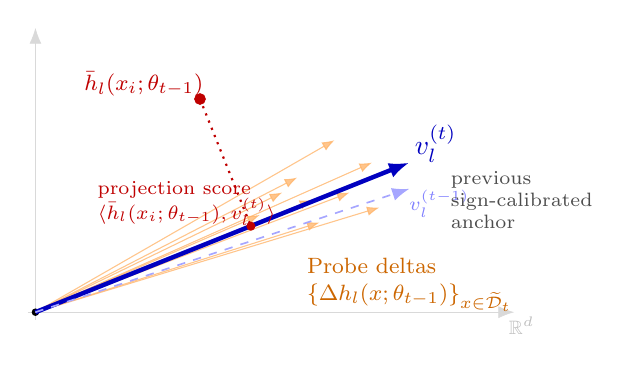
\begin{tikzpicture}[scale=0.95, every node/.style={font=\small}]
  \draw[gray!30, very thin, -{Latex[length=2mm]}] (-0.1,0) -- (6.4,0);
  \draw[gray!30, very thin, -{Latex[length=2mm]}] (0,-0.1) -- (0,3.8);
  \node[gray!50, font=\scriptsize] at (6.5,-0.18) {$\mathbb{R}^d$};

  \filldraw[black] (0,0) circle (1.2pt);

  \foreach \x/\y in
    {3.8/1.2, 4.2/1.6, 3.5/1.8, 4.5/2.0, 3.0/1.3, 4.0/2.3, 3.7/1.5, 4.6/1.4, 3.3/1.6}
  {
    \draw[-{Latex[length=1.6mm]}, orange!60, thin, opacity=0.75]
      (0,0) -- (\x,\y);
  }

  \node[orange!80!black, font=\footnotesize, align=left, anchor=north west] at (3.5,0.85)
    {Probe deltas\\
     $\{\Delta h_l(x;\theta_{t-1})\}_{x\in\widetilde{\mathcal{D}}_t}$};

  \draw[-{Latex[length=2.6mm]}, blue!75!black, ultra thick]
    (0,0) -- (5.0,2.0);
  \node[blue!75!black, font=\bfseries] at (5.35,2.25) {$v_l^{(t)}$};

  \draw[-{Latex[length=2.2mm]}, blue!35, dashed, semithick]
    (0,0) -- (5.0,1.65);
  \node[blue!50, font=\scriptsize] at (5.40,1.45) {$v_l^{(t-1)}$};

  \node[gray!60!black, font=\scriptsize, align=left] at (6.5,1.5)
    {previous\\
     sign-calibrated\\
     anchor};

  \filldraw[red!75!black] (2.2,2.85) circle (2pt);
  \node[red!75!black, font=\footnotesize] at (1.45,3.05)
    {$\bar h_l(x_i;\theta_{t-1})$};

  \draw[red!75!black, dotted, thick] (2.2,2.85) -- (2.88,1.15);
  \filldraw[red!75!black] (2.88,1.15) circle (1.5pt);

  \node[red!75!black, font=\scriptsize, align=left, anchor=west]
    at (0.70,1.45)
    {projection score\\[-1pt]
     $\langle \bar h_l(x_i;\theta_{t-1}), v_l^{(t)}\rangle$};
\end{tikzpicture}

\caption{\textbf{State-conditioned representation anchor at refresh
step~\(t\).}
\textnormal{One-layer schematic. \(\Delta h_l\): probe
representation displacements;
\(v_l^{(t)}\): current anchor; \(v_l^{(t-1)}\): previous anchor;
\(\bar h_l(x_i;\theta_{t-1})\): candidate mean activation. Dotted
line: the layer-wise projection contribution
\(\langle \bar h_l(x_i;\theta_{t-1}), v_l^{(t)}\rangle\), which is
summed in Eq.~\eqref{eq:raw-anchor-projection} to form the raw
anchor-projection score \(a_i^{(t)}\).}}
\label{fig:anchor}
\end{figure}


\subsection{Anchor stability: local analysis and empirical
verification}
\label{sec:local-anchor-stability}

\paragraph{Local stability bound.}
The following Davis--Kahan-style bound records the local sensitivity
of the recomputed PCA anchor. It is used only to motivate the
diagnostic evaluated below; the algorithm itself does not use this
bound.

\begin{theorem}[State-conditioned anchor stability]
\label{thm:anchor-stability}
For notational simplicity, write
\(\Sigma_l^{(t)}=\widehat{\Sigma}_l^{(t)}\), and let \(\eta_{t-1}\)
denote the optimizer learning rate in effect at refresh step \(t\).
Suppose that, for layer \(l\) at refresh step \(t\),
\begin{equation}
  \left\|
  \Sigma_l^{(t)}-\Sigma_l^{(t-1)}
  \right\|_F
  \le
  C_{\Sigma,l}\eta_{t-1},
  \label{eq:cov-drift-assumption}
\end{equation}
and
\begin{equation}
  \lambda_1(\Sigma_l^{(t)})
  -
  \lambda_2(\Sigma_l^{(t-1)})
  \ge
  \gamma_l>0 .
  \label{eq:gap-assumption}
\end{equation}
Under the temporal sign-calibration convention
\(\langle v_l^{(t)},v_l^{(t-1)}\rangle\ge 0\), the anchor displacement
satisfies
\begin{equation}
  \left\|
  v_l^{(t)}-v_l^{(t-1)}
  \right\|_2
  \le
  \frac{2C_{\Sigma,l}}{\gamma_l}\eta_{t-1}.
  \label{eq:anchor-stability-bound}
\end{equation}
\end{theorem}

The proof and the cross-time eigengap convention are deferred to
Appendix~\ref{app:proof-stability}. The bound is conditional: its
constants depend on the realized covariance trajectory, so it is not
a training-time certificate, and it says nothing about candidate
projections or the full ranking. What it does supply is an
observable prediction---anchor displacement at the optimizer
scale---which we now check on a realized trajectory using a
post-hoc verifier that re-extracts each layer's anchor at fixed
intervals during training (protocol below).

\paragraph{Step-to-step anchor displacement.}
\label{sec:empirical-anchor-stability}
For each retained layer \(l\) and consecutive refreshes
\(t-1\!\to\!t\), we measure the step-to-step anchor displacement
\begin{equation}
  d_l^{(t)}
  :=
  \left\|
  v_l^{(t)}-v_l^{(t-1)}
  \right\|_2 ,
  \label{eq:dstep}
\end{equation}
where \(v_l^{(t)}\) denotes the verifier-extracted anchor after
adjacent-refresh sign calibration. Equivalently, if
\(\tilde v_l^{(t)}\) denotes the raw uncalibrated top eigenvector, then
\begin{equation}
  d_l^{(t)}
  =
  \min_{\sigma\in\{\pm1\}}
  \left\|
  \tilde v_l^{(t)}
  -
  \sigma \tilde v_l^{(t-1)}
  \right\|_2
  =
  \sqrt{
  2
  -
  2
  \left|
  \left\langle
  \tilde v_l^{(t)},\tilde v_l^{(t-1)}
  \right\rangle
  \right|
  } .
  \label{eq:dstep-sign-invariant}
\end{equation}
Thus \(d_l^{(t)}\in[0,\sqrt{2}]\). Small values indicate that the
anchor direction is stable across refreshes, while values near
\(\sqrt{2}\) indicate nearly orthogonal consecutive anchors even
after sign calibration. Under the assumptions of
Theorem~\ref{thm:anchor-stability}, the same transition obeys the
bound in Eq.~\eqref{eq:anchor-stability-bound}. We use
\(d_l^{(t)}\) only as a post-hoc diagnostic; it is not used by
Algorithm~\ref{alg:tag} to rank candidates or select data.

\paragraph{Diagnostic protocol.}
We apply a post-hoc verifier to Qwen2.5-0.5B + LoRA training on
Alpaca-GPT4, a small instrumented setting chosen so that per-refresh
anchor extraction over all layers is affordable. Every 25 optimizer
steps, the verifier re-extracts each layer's anchor from a fixed
2,000-sample diagnostic probe and records \(d_l^{(t)}\). This probe
is fixed across refreshes and separate from the resampled
training-time probe \((n_p=1024)\), so \(d_l^{(t)}\)
removes cross-refresh probe-sampling variance and reduces finite-sample
eigenvector noise.

We discard the first 9 refreshes as warm-up and exclude boundary
layers 1 and 24, whose representation displacements are dominated by
embedding-adjacent and output-projection effects. Empirically, these
effects produce near-degenerate local covariance spectra, weakening the
spectral-separation premise of Theorem~\ref{thm:anchor-stability}. The
diagnostic is therefore evaluated on 22 inner decoder layers over 68
post-warmup transitions, giving \(22\times68=1{,}496\) valid
layer--refresh pairs. The global plug-in envelope
\((2\widehat C_{\Sigma}/\gamma_{\min})\eta=46.24\) is too conservative
to be informative at the scale of \(d_l^{(t)}\), as it exceeds the
maximum sign-calibrated displacement \(\sqrt{2}\). The meaningful
comparison is the trajectory-aware Davis--Kahan envelope of
Fig.~\ref{fig:anchor-drift}, which accumulates realized
per-transition drift-to-gap ratios into an upper envelope on the
remaining drift to the final anchor,
\(\|v_l^{(t)}-v_l^{(T)}\|\); its construction is given in
Appendix~\ref{app:anchor-stability-diagnostics}. The measured
\textsc{TAG} drift stays roughly two orders of magnitude below this
envelope throughout training. Unlike
Table~\ref{tab:dstep-spread}, which aggregates only the
\(22\times68\) retained pairs, the figure traces the full
24-layer, 78-point trajectory including warm-up, so the two views
are complementary rather than identical.

\begin{table}[t]
\centering
\caption{Anchor-displacement diagnostic for \textsc{TAG} and matched
CO~\((\lambda{=}0)\). The invariant statistic is
\(d_l^{(t)}\in[0,\sqrt{2}]\). Med. and peak are transition-level layer
summaries aggregated over post-warmup refreshes; worst step is the
maximum retained layer--refresh pair.}
\label{tab:dstep-spread}

\small
\setlength{\tabcolsep}{4pt}
\begin{tabular}{@{}lccccc@{}}
\toprule
 & \multicolumn{2}{c}{\(d^{(t)}\) over layers}
 & worst & sign-flip & \\
\cmidrule(lr){2-3}
Method & med. & peak & step & rate & Status \\
\midrule
\textsc{TAG} \((\lambda=1)\)
 & \(0.034\) & \(0.166\) & \(0.623\) & \(1.7\%\) & \textbf{PASS} \\
CO \((\lambda=0)\)
 & \(0.215\) & \(0.527\) & \(1.405\) & \(\mathbf{11.8\%}\) & \textbf{FAIL} \\
\bottomrule
\end{tabular}
\end{table}

\begin{figure}[t]
\centering
\resizebox{0.97\columnwidth}{!}{%
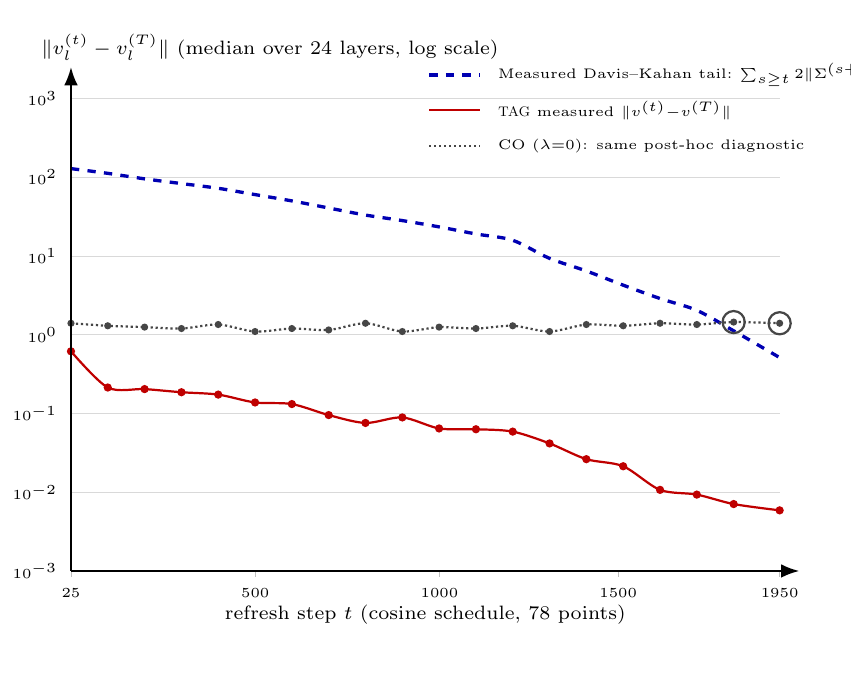
\begin{tikzpicture}[
  every node/.style={font=\scriptsize},
  >=Latex
]


\path[use as bounding box] (-0.55,-0.95) rectangle (9.55,6.90);

% Y-axis grid lines.
\foreach \logv/\ylab in {-3/$10^{-3}$, -2/$10^{-2}$, -1/$10^{-1}$,
                          0/$10^{0}$,  1/$10^{1}$,   2/$10^{2}$, 3/$10^{3}$} {
  \pgfmathsetmacro{\ycoord}{\logv + 3}
  \draw[gray!30, very thin] (0, \ycoord) -- (9, \ycoord);
  \node[anchor=east, font=\tiny] at (-0.05, \ycoord) {\ylab};
}

% X-axis tick labels.
\foreach \step/\xc in {25/0.00, 500/2.34, 1000/4.68, 1500/6.95, 1950/9.00} {
  \draw[gray!50, very thin] (\xc, 0) -- (\xc, -0.08);
  \node[anchor=north, font=\tiny] at (\xc, -0.10) {\step};
}

% Measured Davis--Kahan cumulative tail bound for TAG.
\draw[blue!70!black, very thick, dashed]
  plot[smooth] coordinates {
    (0.000,5.11) (0.467,5.05) (0.935,4.98) (1.403,4.92) (1.870,4.86)
    (2.338,4.78) (2.805,4.70) (3.273,4.61) (3.740,4.52) (4.208,4.45)
    (4.675,4.37) (5.143,4.28) (5.610,4.20) (6.078,3.97) (6.545,3.81)
    (7.013,3.63) (7.481,3.46) (7.948,3.31) (8.416,3.05) (9.000,2.71)
  };

% Matched CO (TAG, lambda=0) control: same post-hoc diagnostic,
% anchor multiplier disabled during selection.
\draw[gray!55!black, thick, densely dotted]
  plot[smooth] coordinates {
    (0.000,3.146) (0.467,3.114) (0.935,3.097) (1.403,3.079) (1.870,3.130)
    (2.338,3.041) (2.805,3.079) (3.273,3.061) (3.740,3.146) (4.208,3.041)
    (4.675,3.097) (5.143,3.079) (5.610,3.114) (6.078,3.041) (6.545,3.130)
    (7.013,3.114) (7.481,3.146) (7.948,3.130) (8.416,3.161) (9.000,3.146)
  };
\foreach \p in {
  (0.000,3.146), (0.467,3.114), (0.935,3.097), (1.403,3.079), (1.870,3.130),
  (2.338,3.041), (2.805,3.079), (3.273,3.061), (3.740,3.146), (4.208,3.041),
  (4.675,3.097), (5.143,3.079), (5.610,3.114), (6.078,3.041), (6.545,3.130),
  (7.013,3.114), (7.481,3.146), (7.948,3.130), (8.416,3.161), (9.000,3.146)
} {
  \fill[gray!55!black] \p circle (1.3pt);
}

% Circle end-of-schedule CO points for diagnostic contrast.
\foreach \p in {(8.416,3.161), (9.000,3.146)} {
  \draw[gray!55!black, thick] \p circle (4.0pt);
}

% TAG measured cumulative drift to final anchor.
\draw[red!75!black, thick]
  plot[smooth] coordinates {
    (0.000,2.79) (0.467,2.33) (0.935,2.31) (1.403,2.27) (1.870,2.24)
    (2.338,2.14) (2.805,2.12) (3.273,1.98) (3.740,1.88) (4.208,1.95)
    (4.675,1.81) (5.143,1.80) (5.610,1.77) (6.078,1.62) (6.545,1.42)
    (7.013,1.33) (7.481,1.03) (7.948,0.97) (8.416,0.85) (9.000,0.77)
  };
\foreach \p in {
  (0.000,2.79), (0.467,2.33), (0.935,2.31), (1.403,2.27), (1.870,2.24),
  (2.338,2.14), (2.805,2.12), (3.273,1.98), (3.740,1.88), (4.208,1.95),
  (4.675,1.81), (5.143,1.80), (5.610,1.77), (6.078,1.62), (6.545,1.42),
  (7.013,1.33), (7.481,1.03), (7.948,0.97), (8.416,0.85), (9.000,0.77)
} {
  \fill[red!75!black] \p circle (1.5pt);
}

% Axes.
\draw[->, thick] (0,0) -- (9.25,0);
\draw[->, thick] (0,0) -- (0,6.40);

\node at (4.50,-0.55)
  {refresh step $t$ (cosine schedule, 78 points)};

\node[anchor=west, align=left, font=\scriptsize] at (-0.50,6.65)
  {\(\|v_l^{(t)} - v_l^{(T)}\|\) (median over 24 layers, log scale)};

% Legend.
\draw[blue!70!black, very thick, dashed] (4.55,6.30) -- (5.20,6.30);
\node[anchor=west, font=\tiny] at (5.30,6.30)
  {Measured Davis--Kahan tail:
  $\sum_{s \ge t} 2\|\Sigma^{(s+1)}{-}\Sigma^{(s)}\|_F/\gamma^{(s)}$};

\draw[red!75!black, thick] (4.55,5.85) -- (5.20,5.85);
\node[anchor=west, font=\tiny] at (5.30,5.85)
  {\textsc{TAG} measured $\|v^{(t)}{-}v^{(T)}\|$};

\draw[gray!55!black, thick, densely dotted] (4.55,5.40) -- (5.20,5.40);
\node[anchor=west, font=\tiny] at (5.30,5.40)
  {CO ($\lambda{=}0$): same post-hoc diagnostic};

\end{tikzpicture}%
}


\caption{\textbf{Representation-anchor stability diagnostic.}
\textnormal{Median layerwise drift to the final anchor,
$\|v_l^{(t)} - v_l^{(T)}\|$ (log scale; $24$ decoder layers,
$78$ cosine-scheduled refresh points; Qwen2.5-0.5B + LoRA).
\emph{Red}: \textsc{TAG} measured drift.
\emph{Blue dashed}: empirical Davis--Kahan tail
$\sum_{s\ge t} 2\|\Sigma^{(s+1)}-\Sigma^{(s)}\|_F/\gamma^{(s)}$.
\emph{Grey dotted}: matched
CO~($\lambda{=}0$) control;
circled markers denote the final two refreshes.}}
\label{fig:anchor-drift}
\end{figure}

\paragraph{Matched Carrier-Only diagnostic.}
We repeat the verifier on a matched Carrier-Only control,
CO~\((\lambda{=}0)\), which removes the anchor factor from the
selection score. CO and \textsc{TAG} share the same cached gate,
optimizer schedule, fixed diagnostic probe, refresh interval, and verifier
protocol; they differ only in the selection score. This matched design separates
representation-anchor modulation from the optimizer schedule and
diagnostic procedure.

For each refresh transition, we summarize \(d_l^{(t)}\) over the
22 retained layers by the layer-wise median and maximum.
Table~\ref{tab:dstep-spread} reports the median over transitions of
these summaries, denoted ``med.'' and ``peak,'' respectively, together
with the worst step \(\max_{l,t}d_l^{(t)}\) over all 1,496 retained
pairs. The sign-flip rate is the fraction of retained pairs satisfying
\(\langle \tilde v_l^{(t)}, v_l^{(t-1)} \rangle < 0\). This rate is
only an orientation diagnostic; the sign-invariant stability statistic
is \(d_l^{(t)}\). For table status, a run passes if no retained pair
exceeds \(d_l^{(t)}=1\), corresponding to a sign-calibrated angle below
\(60^\circ\). This descriptive criterion is not a theorem-level
guarantee; it flags transitions approaching the near-orthogonal regime.
The contrast in Table~\ref{tab:dstep-spread} is descriptive but
informative: the \textsc{TAG} trajectory stays well inside the stable
regime, while the carrier-only trajectory repeatedly approaches
near-orthogonal anchor transitions. The stability that the bounded
modulation relies on is thus a property the anchored run empirically
maintains, not merely an assumption.


\subsection{Fused score: a zero-anchored product rule}
\label{sec:tag-score}

Equation~\eqref{eq:tag-score-method} fuses the three views
multiplicatively. The product form itself is classical---product-rule
and log-opinion-pool combination of evidence goes back at least to
combining-classifier and expert-aggregation
theory~\cite{kittler1998combining,genest1986combining}---and in log
space the score is simply the additive pool
\(\log s_i^{(t)}=\log G_i+\log\mathcal R_i^{(t)}
+\log\bigl(1+\lambda\,\widetilde a_i^{(t)}\bigr)\).
What the design contributes is the deliberate \emph{asymmetry of the
three roles} within that pool. The gate is absolute and
zero-anchored: \(G_i=0\) annihilates the score and, via the
selection key of Eq.~\eqref{eq:tag-selection-key}, cannot be
re-admitted ahead of any positive-gate candidate, whatever the
dynamic terms---the veto is non-compensatory. Additive or
averaging fusion cannot provide this behavior: a sufficiently large
utility term always outweighs a zero reliability score,
re-admitting exactly the corrupted-but-difficult candidates the
gate exists to remove. The same point separates the design from
trusted multi-view classification, which re-weights or averages
conflicting views~\cite{tmc2021,rcml2024}: in data selection,
unreliability must be able to reach the floor, not merely lose
weight. The two dynamic factors are, by design, weaker: the carrier
\(\mathcal R_i^{(t)}\) is pool-relative and carries the dynamic
ranking, while the anchor factor is confined to
\([1,1+\lambda]\), so it modulates the carrier by at most a factor
of \(1{+}\lambda\) and can neither veto nor dominate. The views
also differ in acquisition schedule---\(G_i\) once at \(\theta_0\),
carrier and anchor at every refresh---so reliability screening adds
no recurring cost. Finally, each view is independently ablatable:
setting \(G_i\equiv 1\) removes the gate without changing the
underlying selector, and setting \(\lambda=0\) removes
representation-anchor modulation, leaving the carrier-only
configuration CO used as the matched control above and as a
baseline in Section~\ref{sec:experiments}.

\subsection{Algorithm and implementation}
\label{sec:algorithm-implementation}

Algorithm~\ref{alg:tag} summarizes the complete procedure. The gate
requires two base-checkpoint forward passes---one under the observed
instruction and one under its counterfactual---and is then cached. Each
refresh uses the current checkpoint only for the reward and anchor.

\begin{algorithm}[t]
  \caption{\textsc{TAG}: reliability-gated training-adaptive selection}
  \label{alg:tag}
  \begin{algorithmic}[1]
  \STATE \textbf{Input:} Pool $\mathcal D$; clean gate reference $\mathcal D_{\mathrm{ref}}$; model $p_{\theta_0}$; budget $B$; anchor strength $\lambda$; refreshes $T$
  \STATE Construct condition-side counterfactuals and compute and cache $G_i$ by Section~\ref{sec:reliability-gate}; see Appendix~\ref{app:gate-implementation}.
  \FOR{$t = 1, \dots, T$}
    \STATE Sample probe $\widetilde{\mathcal D}_t\subset\mathcal D$ uniformly.
    \STATE Under $\theta_{t-1}$, compute $\mathcal L_i^{(t)}$, $\mathcal H_i^{(t)}$, and the hidden states required by the anchor.
    \STATE Compute $\mathcal R_i^{(t)}$ by Eqs.~\eqref{eq:composite}--\eqref{eq:w}.
    \STATE Update $v_l^{(t)}$ and $\widetilde a_i^{(t)}$ by Eqs.~\eqref{eq:anchor-delta-mean}--\eqref{eq:anchor-projection-norm}.
    \STATE $s_i^{(t)}\gets G_i\mathcal R_i^{(t)}\bigl(1+\lambda\widetilde a_i^{(t)}\bigr)$.
    \STATE $\mathcal S_t\gets$ top-$B$ candidates by the key $\kappa_i^{(t)}$ of Eq.~\eqref{eq:tag-selection-key}.
    \STATE Fine-tune $\theta_{t-1}\to\theta_t$ on $\mathcal S_t$.
  \ENDFOR
  \STATE \textbf{return} $\theta_T$
  \end{algorithmic}
\end{algorithm}

% =====================================================================
%  Section 4: Experiments
%  Main setting: LLaMA-2-7B full fine-tuning, Alpaca-GPT4,
%  10% selection, nine evaluation tasks across five capability groups.
% =====================================================================
\section{Experiments}
\label{sec:experiments}

\begin{table*}[t]
\centering
\begin{threeparttable}
\caption{\textbf{Performance comparison of baselines using 10\% of
the IT data.} This table shows the results of various tasks across
multiple baselines. \textbf{Bold} and \underline{underline} represent the best and 
second-best performance respectively in each column 
\emph{among 10\% selection methods (R10, ID~02--09);} ID~00 and 
ID~01 are shown as lower/upper-bound references and excluded 
from the ranking. $\Delta\,(\uparrow)$ indicates the performance improvement
relative to ID~01.}
\label{tab:main-results}
\small
\setlength{\tabcolsep}{2.9pt}
\renewcommand{\arraystretch}{1.01}

\begin{tabular}{@{}llcccccccccc@{}}
\toprule
 & &
 \multicolumn{2}{c}{Knowledge \& reasoning} &
 \multicolumn{2}{c}{Math} &
 \multicolumn{2}{c}{Code} &
 \multicolumn{2}{c}{Multilingual QA} &
 \multicolumn{2}{c}{Overall} \\
\cmidrule(lr){3-4}
\cmidrule(lr){5-6}
\cmidrule(lr){7-8}
\cmidrule(lr){9-10}
\cmidrule(lr){11-12}
ID & Method
& \shortstack[c]{MMLU\\[-1pt]{\scriptsize exam}}
& \shortstack[c]{BBH\\[-1pt]{\scriptsize hard tasks}}
& \shortstack[c]{SVAMP\\[-1pt]{\scriptsize robust math}}
& \shortstack[c]{GSM8K\\[-1pt]{\scriptsize grade math}}
& \shortstack[c]{MBPP\\[-1pt]{\scriptsize program}}
& \shortstack[c]{H-Eval\\[-1pt]{\scriptsize function}}
& \shortstack[c]{TydiQA\\[-1pt]{\scriptsize 9-lang F1}}
& \shortstack[c]{XQuAD\\[-1pt]{\scriptsize 12-lang F1}}
& \shortstack[c]{AVG\\[-1pt]{\scriptsize 8-task mean}}
& \shortstack[c]{$\Delta$\\[-1pt]{\scriptsize vs Full FT}} \\
\midrule

\rowcolor{gray!15}
\multicolumn{12}{@{}l}{\textbf{Data-side references}}\\
00 & Pure LLaMA-2-7B (No FT)
    & 45.82 & 36.35
    & 36.67 & 13.87
    & 0.00$^\dagger$ & 2.38$^\dagger$
    & 61.70 & 55.08
    & 31.48 & $-20.96\%$ \\
01 & Alpaca-GPT4 (Full FT)
    & 47.86 & 37.19
    & 40.33 & 16.60
    & 37.35 & 25.60
    & 60.74 & 52.99
    & 39.83 & --- \\
R10 & Random ($10\%$)
    & 45.04 & 35.54
    & 36.80 & 13.57
    & 35.41 & 24.51
    & \underline{60.83} & 52.28
    & 38.00 & $-4.61\%$ \\
\midrule
\rowcolor{gray!15}
\multicolumn{12}{@{}l}{\textbf{Static 10\% IT-data selection}}\\
02 & LIMA
    & 46.44 & 36.68
    & 36.20 & 16.38
    & 33.07 & 22.09
    & 59.28 & 51.14
    & 37.66 & $-5.45\%$ \\
03 & AlpaGasus
    & 46.17 & 36.36
    & 38.33 & 16.22
    & 37.50 & 23.94
    & 60.81 & \underline{53.87}
    & 39.15 & $-1.71\%$ \\
04 & Q2Q
    & 46.18 & 36.84
    & 34.33 & \underline{17.82}
    & 36.19 & 25.19
    & 60.42 & 52.34
    & 38.66 & $-2.93\%$ \\
05 & SelectIT
    & 46.02 & 38.37
    & 36.33 & 16.98
    & 36.58 & \underline{28.17}
    & 60.44 & \textbf{54.12}
    & 39.63 & $-0.52\%$ \\
06 & NAIT (All)
    & 46.08 & 40.02
    & \underline{39.67} & 17.06
    & 35.41 & 26.44
    & 60.03 & 52.87
    & 39.70 & $-0.34\%$ \\
\midrule
\rowcolor{gray!15}
\multicolumn{12}{@{}l}{\textbf{Dynamic 10\% selection}}\\
07 & \textsc{Data Agent (PPO)}
    & \underline{46.49} & 38.37
    & 37.67 & 16.48
    & \textbf{39.69} & \textbf{28.61}
    & 60.44 & 50.85
    & \underline{39.83} & \underline{$-0.02\%$} \\
08 & CO ($\lambda=0$)
    & 45.90 & \underline{40.21}
    & 36.67 & 16.53
    & 34.63 & 24.38
    & 60.12 & 50.70
    & 38.64 & $-2.99\%$ \\
\rowcolor{red!8}
09 & \textbf{\textsc{TAG}} ($\lambda=1$)
    & \textbf{47.71} & \textbf{40.36}
    & \textbf{40.33} & \textbf{18.27}
    & \underline{38.52} & 25.87
    & \textbf{61.13} & 53.43
    & \textbf{40.70} & \textbf{$+2.18\%$} \\
\bottomrule
\end{tabular}
\begin{tablenotes}[flushleft]
\footnotesize
\item[$\dagger$] MBPP grades pass@1 by executing the generated
function; the non-instruction-tuned base model emits free-form
text instead of parseable code, yielding $0$. HumanEval is a
signature+docstring completion task closer to pretraining, hence
the near-zero $2.38$.
\end{tablenotes}
\end{threeparttable}
\end{table*}

We evaluate \textsc{TAG} as a dynamic re-ranking method for
instruction-tuning data selection. Our primary setting is
full-parameter fine-tuning of LLaMA-2-7B~\cite{touvron2023llama2} on
Alpaca-GPT4~\cite{wang2023selfinstruct} with a fixed selection budget
of \(\rho{=}10\%\). Robustness experiments additionally vary the
backbone, using Qwen2.5-0.5B, Qwen2.5-7B~\cite{qwen2025technical},
and Mistral-7B~\cite{jiang2023mistral}, and the source dataset, using
WizardLM Evol-Instruct~\cite{xu2024wizardlm}. Within each
(backbone, dataset) setting, all selectors share the same training
hyperparameters and evaluation protocol; only the selected subset
differs. Full FT uses the full pool, while all selection methods use
\(10\%\), a budget chosen because random ratio sweeps show that
increasing random subsets up to \(50\%\) provides little additional
headroom.

We evaluate eight benchmarks spanning four capability families:
knowledge and hard reasoning (MMLU, BBH), mathematical reasoning
(SVAMP, GSM8K), code generation (MBPP, HumanEval), and multilingual QA
(TyDiQA, XQuAD). We report per-task scores, AVG, and \(\Delta\) over
Full FT; benchmark scoring conventions are summarized in the appendix.

\paragraph{Baselines.}
We compare against Full FT, random subsets, static instruction-data
selectors (LIMA, AlpaGasus, Q2Q, SelectIT, NAIT), the PPO-based Data
Agent, and CO, the Carrier-Only variant obtained by setting
\(\lambda{=}0\). CO is the direct baseline for isolating the
contribution of representation-anchor modulation.

\paragraph{Research questions.}
The experiments ask whether \textsc{TAG} (i) outperforms static and
dynamic selectors at the same \(10\%\) budget, (ii) remains robust
across backbones and source datasets, (iii) has a stable
anchor-strength choice, and (iv) adds only modest re-ranking overhead.


% \subsection{Main result}
% \label{sec:main-result}

% Table~\ref{tab:main-results} reports the main comparison under the same
% selection budget and evaluation protocol. The controlled comparison
% between the carrier-only baseline (CO) and \textsc{TAG} isolates the
% effect of representation-anchor modulation: both use the same dynamic re-ranking
% pipeline and carrier reward, while \textsc{TAG} additionally enables
% the anchor term. The key quantitative result is that \textsc{TAG}
% reaches an 8-task AVG of 40.70, the highest overall score among all
% 10\% selection methods.

% \paragraph{Effect of representation-anchor modulation.}
% \textsc{TAG} consistently improves over the CO baseline across the
% benchmark suite. Quantitatively, the anchor raises AVG from 38.64 to
% 40.70 (+2.06 pp), with especially clear gains on MBPP (+3.89 pp),
% SVAMP (+3.66 pp), and XQuAD (+2.73 pp). The gains span reasoning,
% math, code, and multilingual QA, suggesting that the anchor does not
% merely specialize selection to one capability family. This supports
% the central claim that a state-conditioned structural signal can
% improve dynamic data selection without seed examples, validation
% labels, or auxiliary scorers.

% \paragraph{Comparison to baselines.}
% Among methods using the same selection budget, \textsc{TAG} achieves
% the strongest overall performance, outperforming static selectors and
% the PPO-based Data Agent. On the same 10\% budget, this corresponds
% to a +0.87 pp gain over the PPO-based Data Agent and a +1.00 pp gain
% over the strongest static selector, NAIT. Static selectors rely on fixed
% or precomputed signals, whereas \textsc{TAG} refreshes a
% model-intrinsic representation signal during training. The random subset
% results serve only as budget controls, separating selection quality
% from the effect of using more data.

% \paragraph{Selection can beat scale.}
% The results show that a carefully selected subset can outperform full
% fine-tuning. In particular, \textsc{TAG} reaches 40.70 with only 10\%
% of the instruction-tuning data, compared with 39.83 for full
% fine-tuning, yielding a +0.87 pp absolute gain and a +2.18\% relative
% improvement. This highlights the value of adaptive selection criteria
% that are not only accurate, but also stable, reference-free, and
% computationally practical.


\subsection{Main result}
\label{sec:main-result}

Table~\ref{tab:main-results} reports the main comparison under the same
selection budget and evaluation protocol. The controlled comparison
between the carrier-only baseline (CO) and \textsc{TAG} isolates
representation-anchor modulation: both use the same dynamic re-ranking
pipeline and carrier reward, while \textsc{TAG} additionally enables
the anchor-projection factor. \textsc{TAG} reaches \textbf{40.70 AVG}, the highest
score among 10\% selection methods.

\paragraph{Effect of representation-anchor modulation.}
\textsc{TAG} consistently improves over the CO baseline across
benchmarks. The anchor raises AVG from 38.64 to 40.70
(+2.06 pp), with clear gains on MBPP (+3.89 pp), SVAMP (+3.66 pp),
and XQuAD (+2.73 pp). The gains span reasoning, math, code, and
multilingual QA, suggesting that the anchor does not merely
specialize to one capability family. This supports our claim that a
state-conditioned representation signal can improve dynamic data
selection without seed examples or auxiliary scorers. Among methods
using the same budget, \textsc{TAG}
achieves the strongest overall performance, outperforming static
selectors and the PPO-based Data Agent. At the same 10\% budget,
\textsc{TAG} gains +0.87 pp over Data Agent and +1.00 pp over
NAIT. Static selectors rely on fixed or precomputed signals, whereas
\textsc{TAG} recomputes its representation anchor from the current
model state at each refresh. The random subset results serve only as
budget controls,
separating selection quality from data scale.

\paragraph{Selection can beat scale.}
The results show that a carefully selected subset can outperform full
fine-tuning. With only 10\% data, \textsc{TAG} scores 40.70 versus
39.83 for Full FT, yielding +0.87 pp absolute and +2.18\% relative
gains. This highlights the value of adaptive selection criteria that
are not only accurate, but also stable, reference-free, and
computationally practical.


\begin{figure}[!ht]
\centering

% ============ TOP: compact Delta plot ============
\resizebox{0.97\columnwidth}{!}{%
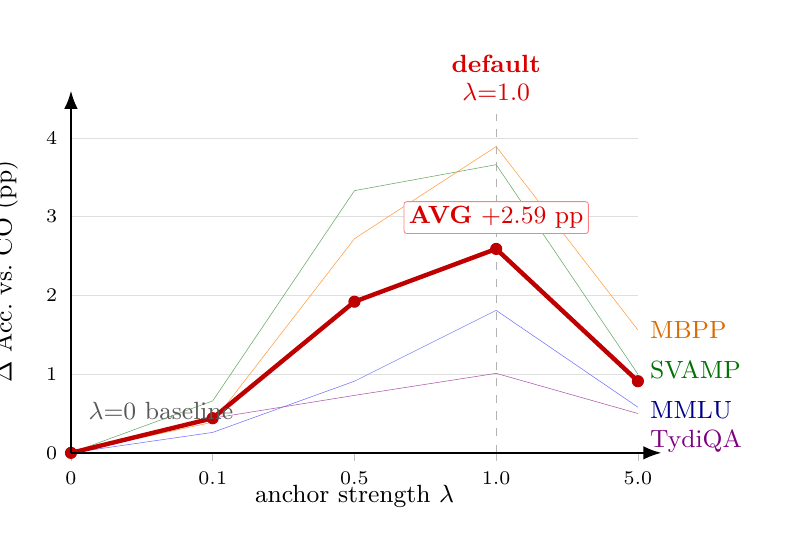
\begin{tikzpicture}[every node/.style={font=\scriptsize}, >=Latex]

\path[use as bounding box] (-0.55,-0.95) rectangle (8.80,5.40);

% Y-axis grid  (왼쪽 숫자 0~4)
\foreach \y in {0,1,2,3,4} {
  \draw[gray!25, very thin] (0,\y) -- (7.2,\y);
  \node[anchor=east, font=\scriptsize] at (-0.05,\y) {\y};
}

% X-axis ticks (0, 0.1, 0.5, 1.0, 5.0)
\foreach \xpos/\lab in
  {0/0, 1.8/0.1, 3.6/0.5, 5.4/1.0, 7.2/5.0} {
  \draw[gray!50, very thin] (\xpos,0) -- (\xpos,-0.10);
  \node[anchor=north, font=\scriptsize] at (\xpos,-0.12) {$\lab$};
}

% Default lambda = 1.0 guideline
\draw[gray!60, dashed, thin] (5.4,0) -- (5.4,4.30);
\node[red!85!black, font=\small, anchor=south, align=center]
  at (5.4,4.35) {\textbf{default}\\[-1pt]$\lambda{=}1.0$};

% Per-task lines
\draw[blue!55, very thin] plot coordinates
  {(0,0) (1.8,0.26) (3.6,0.91) (5.4,1.81) (7.2,0.58)};
\draw[green!45!black!60, very thin] plot coordinates
  {(0,0) (1.8,0.66) (3.6,3.33) (5.4,3.66) (7.2,1.00)};
\draw[orange!75, very thin] plot coordinates
  {(0,0) (1.8,0.39) (3.6,2.72) (5.4,3.89) (7.2,1.56)};
\draw[violet!65, very thin] plot coordinates
  {(0,0) (1.8,0.44) (3.6,0.73) (5.4,1.01) (7.2,0.50)};

% Endpoint labels (좁은 구간에 모여있어 강제 분산)
\node[orange!85!black,font=\small, anchor=west] at (7.23,1.56) {MBPP};
\node[green!45!black, font=\small, anchor=west] at (7.23,1.05) {SVAMP};
\node[blue!55!black,  font=\small, anchor=west] at (7.23,0.55) {MMLU};
\node[violet,         font=\small, anchor=west] at (7.23,0.15) {TydiQA};

% Average line (굵게)
\draw[red!75!black, ultra thick] plot coordinates
  {(0,0) (1.8,0.44) (3.6,1.92) (5.4,2.59) (7.2,0.91)};
\foreach \p in {(0,0), (1.8,0.44), (3.6,1.92),
                (5.4,2.59), (7.2,0.91)} {
  \fill[red!75!black] \p circle (2.2pt);
}

% Best average callout (Avg. 라벨을 callout에 통합)
\node[red!85!black, font=\small, anchor=south,
      fill=white, draw=red!50, line width=0.3pt,
      rounded corners=1pt, inner sep=1.8pt]
  at (5.4,2.78) {\textbf{AVG}\ $+2.59$ pp};
% Baseline note
\node[gray!70!black, font=\small, anchor=south west]
  at (0.1,0.3) {$\lambda{=}0$ baseline};

% Axes
\draw[->, thick] (0,0) -- (7.50,0);
\draw[->, thick] (0,0) -- (0,4.60);

% X-axis title
\node[font=\small] at (3.60,-0.55)
  {anchor strength $\lambda$};
% Y-axis title
\node[font=\small, rotate=90, anchor=south] at (-0.55,2.30)
  {$\Delta$ Acc.\ vs.\ CO (pp)};
\end{tikzpicture}%
}

\vspace{0.45em}

% ============ BOTTOM: compact table ============
{\fontsize{8pt}{12pt}\selectfont
\setlength{\tabcolsep}{3pt}

\begin{tabularx}{0.97\columnwidth}{@{}l*{5}{>{\centering\arraybackslash}X}@{}}
\toprule
$\lambda$ & MMLU & SVAMP & MBPP & TydiQA & AVG \\
\midrule
$0$ (CO)
 & $45.90$
 & $36.67$
 & $34.63$
 & $60.12$
 & $44.33$ \\

$0.1$
 & \shortstack[c]{$46.16$\\[-1pt]{\scriptsize$(+0.26)$}}
 & \shortstack[c]{$37.33$\\[-1pt]{\scriptsize$(+0.66)$}}
 & \shortstack[c]{$35.02$\\[-1pt]{\scriptsize$(+0.39)$}}
 & \shortstack[c]{$60.56$\\[-1pt]{\scriptsize$(+0.44)$}}
 & \shortstack[c]{$44.77$\\[-1pt]{\scriptsize$(+0.44)$}} \\

$0.5$
 & \shortstack[c]{$46.81$\\[-1pt]{\scriptsize$(+0.91)$}}
 & \shortstack[c]{$40.00$\\[-1pt]{\scriptsize$(+3.33)$}}
 & \shortstack[c]{$37.35$\\[-1pt]{\scriptsize$(+2.72)$}}
 & \shortstack[c]{$60.85$\\[-1pt]{\scriptsize$(+0.73)$}}
 & \shortstack[c]{$46.25$\\[-1pt]{\scriptsize$(+1.92)$}} \\

\rowcolor{red!8}
$\mathbf{1.0}$
 & \shortstack[c]{$\mathbf{47.71}$\\[-1pt]{\scriptsize$(+1.81)$}}
 & \shortstack[c]{$\mathbf{40.33}$\\[-1pt]{\scriptsize$(+3.66)$}}
 & \shortstack[c]{$\mathbf{38.52}$\\[-1pt]{\scriptsize$\mathbf{(+3.89)}$}}
 & \shortstack[c]{$\mathbf{61.13}$\\[-1pt]{\scriptsize$(+1.01)$}}
 & \shortstack[c]{$\mathbf{46.92}$\\[-1pt]{\scriptsize$\mathbf{(+2.59)}$}} \\

$5.0$
 & \shortstack[c]{$46.48$\\[-1pt]{\scriptsize$(+0.58)$}}
 & \shortstack[c]{$37.67$\\[-1pt]{\scriptsize$(+1.00)$}}
 & \shortstack[c]{$36.19$\\[-1pt]{\scriptsize$(+1.56)$}}
 & \shortstack[c]{$60.62$\\[-1pt]{\scriptsize$(+0.50)$}}
 & \shortstack[c]{$45.24$\\[-1pt]{\scriptsize$(+0.91)$}} \\
\bottomrule
\end{tabularx}
}

\caption{\textbf{$\lambda$-ablation of the anchor-modulation
strength.}
LLaMA-2-7B + Alpaca-GPT4 at $\rho{=}10\%$. Gains are reported over the
CO baseline, obtained by disabling representation-anchor modulation
($\lambda{=}0$). The sweep shows an inverted-U trend, with
$\lambda{=}1.0$ serving as our empirical default.}
\label{fig:lambda-ablation}
\end{figure}

\subsection{$\lambda$-ablation of the anchor-modulation strength}
\label{sec:lambda-ablation}
\paragraph{Inverted-U effect of anchor modulation.}
Figure~\ref{fig:lambda-ablation} shows an inverted-U effect. When
\(\lambda{=}0\), the method removes representation-anchor modulation
and recovers the CO baseline to within noise. As \(\lambda\) grows,
high-projection candidates exert increasing influence on the carrier
ranking; beyond \(\lambda{=}1\), the gains decline. This pattern
supports using the projection as a bounded auxiliary signal rather
than allowing it to dominate the carrier.

\paragraph{Default choice of \(\lambda{=}1.0\).}
The sweep peaks at \(\lambda{=}1.0\), and this optimum is stable across
tasks and backbones. We therefore use \(\lambda{=}1.0\) as the
empirical default and expose only \(\rho\) in the remaining
experiments.



% ============== Table 4: Efficiency and dependency comparison ==============
% No package required for the symbols below.
\providecommand{\nodep}{--}
\providecommand{\paiddep}{\textbf{\$}}
\providecommand{\seeddep}{\textsc{Seed}}
\providecommand{\humandep}{\textsc{Human}}
\providecommand{\notmeasured}{\textsc{N/M}$^{\dagger}$}
\providecommand{\costlb}[1]{$>#1^{\dagger}$}

\begin{table}[t]
\centering
\caption{\textbf{Cost and dependency comparison} at
$\rho{=}10\%$ on LLaMA-2-7B + Alpaca-GPT4.}
\label{tab:efficiency}

{\fontsize{8pt}{11pt}\selectfont
\setlength{\tabcolsep}{3pt}

\begin{tabularx}{\columnwidth}{@{}Yccrrr@{}}
\toprule
Method
& \shortstack[c]{Ext.\\[-1pt]Scorer}
& \shortstack[c]{Cap.\\[-1pt]Ref.}
& \shortstack[c]{Sel.\\[-1pt]h}
& \shortstack[c]{SFT\\[-1pt]h}
& \shortstack[c]{Cost\\[-1pt]\$} \\
\midrule

\rowcolor{gray!15}
\multicolumn{6}{@{}l@{}}{\textbf{Static / precomputed selectors}}\\
LIMA       & \humandep & \nodep & \notmeasured & 0.28 & \costlb{0.33} \\
AlpaGasus  & \paiddep  & \nodep & \notmeasured & 0.63 & \costlb{0.73} \\
Q2Q        & \paiddep  & \nodep & \notmeasured & 0.62 & \costlb{0.71} \\
SelectIT   & \nodep    & \nodep & \notmeasured & 0.64 & \costlb{0.74} \\

\midrule

\rowcolor{gray!15}
\multicolumn{6}{@{}l@{}}{\textbf{Static / model-internal selector}}\\
NAIT       & \nodep & \seeddep & 1.18 & 0.66 & 2.11 \\

\midrule

\rowcolor{gray!15}
\multicolumn{6}{@{}l@{}}{\textbf{Dynamic / model-internal selectors}}\\
Data Agent (PPO) & \nodep & \nodep & 3.77 & 0.68 & 5.11 \\

\rowcolor{red!8}
\textbf{\textsc{TAG} (ours)}
& \nodep & \nodep
& \textbf{2.34}
& \textbf{0.64}
& \textbf{3.43} \\

\bottomrule
\end{tabularx}
}

\vspace{2pt}
\begin{minipage}{\columnwidth}
\footnotesize
\textit{Notes.} ``--'' denotes no dependency;
\humandep/\paiddep: human/paid-API scoring;
\seeddep: human-chosen in-domain seed.
GPU cost measured on A100 80GB at effective batch $128$,
normalized at \$$1.15$/A100-hr. $^{\dagger}$~SFT cost only;
selection stage not measured in our local setup. For API-based
selectors (AlpaGasus, Q2Q), API cost depends on scorer model,
candidate count, and prompt/output length (GPT-4.1 rates:
\$$2.00$/M input, \$$8.00$/M output tokens).
\end{minipage}
\end{table}

% ============== Table 5: Backbone robustness ==============

\begin{table}[t]
\centering
\caption{\textbf{Multi-backbone robustness on Alpaca-GPT4 (0.5B--7B).}}
\label{tab:backbone-robustness}
{\fontsize{8pt}{11pt}\selectfont
\setlength{\tabcolsep}{3pt}
\begin{tabularx}{\columnwidth}{@{}Yrrrrr@{}}
\toprule
Method & MMLU & SVAMP & MBPP & TydiQA & AVG \\
\midrule
\rowcolor{gray!15}
\multicolumn{6}{@{}l@{}}{\textbf{Mistral-7B}} \\
Full FT (100\%)        & 53.13              & \underline{58.24} & \textbf{51.22}     & 50.16              & 53.19 \\
Random (10\%)          & 56.80              & 57.00              & 48.64              & \underline{53.29}  & 53.93 \\
Data Agent (PPO, 10\%) & \underline{57.38}  & 56.67              & 50.28              & \textbf{54.36}     & \underline{54.67} \\
\rowcolor{red!8}
\textbf{\textsc{TAG} ($\lambda{=}1$, 10\%)} & \textbf{57.93} & \textbf{61.33} & \underline{50.97} & 53.09 & \textbf{55.83} \\
\addlinespace[3pt]

\rowcolor{gray!15}
\multicolumn{6}{@{}l@{}}{\textbf{Qwen2.5-7B}} \\
Full FT (100\%)        & \textbf{73.93}     & \underline{83.33} & 74.31              & \underline{55.78}  & \underline{71.84} \\
Random (10\%)          & 71.92              & 83.00              & \textbf{75.48}     & 54.10              & 71.13 \\
Data Agent (PPO, 10\%) & 73.59              & 83.01              & \textbf{75.48}     & 53.66              & 71.43 \\
\rowcolor{red!8}
\textbf{\textsc{TAG} ($\lambda{=}1$, 10\%)} & \underline{73.68} & \textbf{83.66} & \underline{75.10} & \textbf{56.83} & \textbf{72.32} \\
\addlinespace[3pt]

\rowcolor{gray!15}
\multicolumn{6}{@{}l@{}}{\textbf{Qwen2.5-0.5B}} \\
Full FT (100\%)        & \textbf{47.85}     & 41.33              & 41.63              & 40.27              & 42.77 \\
Random (10\%)          & 47.71              & 40.68              & 43.19              & 39.88              & 42.87 \\
Data Agent (PPO, 10\%) & 47.46              & \underline{44.00} & \underline{46.30} & \underline{41.04} & \underline{44.70} \\
\rowcolor{red!8}
\textbf{\textsc{TAG} ($\lambda{=}1$, 10\%)} & \underline{47.77} & \textbf{45.33} & \textbf{47.08} & \textbf{42.73} & \textbf{45.73} \\
\bottomrule
\end{tabularx}
}
\end{table}

% ============== Table 6: Instruction-dataset transfer (Evol-Instruct) ==============
\begin{table}[t]
\centering
\caption{\textbf{Instruction-dataset transfer on Evol-Instruct} at $\rho{=}10\%$.  Setup mirrors Table~\ref{tab:backbone-robustness}}
\label{tab:dataset-transfer}
{\fontsize{8pt}{12pt}\selectfont
\setlength{\tabcolsep}{3pt}
\begin{tabularx}{\columnwidth}{@{}Yrrrrr@{}}
\toprule
Method & MMLU & SVAMP & MBPP & TydiQA & AVG \\
\midrule
\rowcolor{gray!15}
\multicolumn{6}{@{}l@{}}{\textbf{LLaMA-2-7B}} \\
Full FT (100\%)        & \underline{45.63} & 37.67 & 35.41 & \underline{64.10} & 45.70 \\
Random (10\%)          & 45.50 & \textbf{38.67} & \textbf{38.52} & 64.00 & \underline{46.67} \\
Data Agent (PPO, 10\%) & 44.89 & 38.27 & \underline{38.44} & 63.65 & 46.31 \\
\rowcolor{red!8}
\textbf{\textsc{TAG} ($\lambda{=}1$, 10\%)} & \textbf{46.25} & \underline{38.45} & 37.69 & \textbf{64.96} & \textbf{46.84} \\
\addlinespace[3pt]
\rowcolor{gray!15}
\multicolumn{6}{@{}l@{}}{\textbf{Qwen2.5-7B}} \\
Full FT (100\%)        & \textbf{71.79} & 81.00 & 75.88 & 57.80 & 71.62 \\
Random (10\%)          & \underline{71.71} & \underline{83.33} & 75.88 & \textbf{59.10} & \textbf{72.51} \\
Data Agent (PPO, 10\%) & 71.02 & 82.74 & \textbf{76.45} & \underline{58.79} & 72.25 \\
\rowcolor{red!8}
\textbf{\textsc{TAG} ($\lambda{=}1$, 10\%)} & 71.68 & \textbf{84.16} & \underline{76.02} & 58.04 & \underline{72.48} \\
    \bottomrule
\end{tabularx}
}
\end{table}

\subsection{Cost of reference-free dynamic selection}
\label{sec:cost}
Table~\ref{tab:efficiency} reports measured local costs and required
dependencies under the same selection budget. ``Cap. ref.'' denotes
a capability reference used to guide selection, such as an in-domain
seed set manually chosen to represent the target capability space.
Static/precomputed selectors are included only as lower-bound
references, since their reported costs do not fully capture offline
dependencies such as external scoring, subset construction, or
curated references.

Among measured model-internal selectors, NAIT is cheaper than
\textsc{TAG}, but it relies on a human-chosen in-domain seed as a
capability reference. This is a strong manual prior: it requires
target-domain knowledge before selection and can bias the selected
subset toward the seed distribution. NAIT's low computational cost
is thus partly obtained by shifting difficulty to manual reference
construction, which is hard to scale, audit, and reproduce.

\textsc{TAG} removes this seed-reference dependency. It is moderately
more expensive than NAIT because state-conditioned dynamic selection
requires additional scoring, but remains cheaper than Data Agent (PPO).
The reason is structural: the carrier and anchor projections reuse
the same scoring pass, so \textsc{TAG} adds lightweight geometric
post-processing rather than a separate policy-optimization loop. Thus,
\textsc{TAG} trades moderate overhead for reference-free dynamic
selection with lower measured cost than the PPO-based selector in our
local setup.


\subsection{Backbone robustness check}
\label{sec:qwen-scale}

Table~\ref{tab:backbone-robustness} evaluates the same \textsc{TAG}
configuration (\(\lambda{=}1,\rho{=}10\%\)) on Alpaca-GPT4 across
Mistral and Qwen backbones spanning 0.5B--7B parameters; AVG averages
MMLU, SVAMP, MBPP, and TyDiQA. \textsc{TAG} achieves the best AVG in
all three backbone groups, suggesting that representation-anchor
modulation is not specific to the LLaMA-2-7B setting.


\subsection{Instruction-dataset transfer}
\label{sec:dataset-transfer}

Table~\ref{tab:dataset-transfer} replaces Alpaca-GPT4 with
WizardLM Evol-Instruct to test transfer across instruction-data
distributions. Evol-Instruct contains harder and more structured
instructions, making random \(10\%\) subsets strong and leaving
less headroom for selection gains.

\textsc{TAG} achieves the best AVG on LLaMA-2-7B. On Qwen2.5-7B,
it nearly ties the best Random baseline while still outperforming
Full FT and Data Agent. Thus, even under a stronger source-data
regime, the same representation-anchor rule remains competitive
without retuning.


\section{Discussion}
\label{sec:discussion}

The central message of \textsc{TAG} is that the utility of a reliable
instruction--response pair depends on the current model state and need
not be captured by a scalar reward alone. We augment the
difficulty--uncertainty carrier with a state-conditioned representation
anchor: principal directions are extracted from the current probe's
within-sequence representation displacements, and normalized candidate
projections provide a bounded multiplicative modulation. This connects
static representation-geometric selection and dynamic scalar-reward
selection under a single ranking rule with one exposed knob,
\(\lambda\).

The theoretical claim is deliberately local. Under covariance-drift
and eigengap conditions, the Davis--Kahan analysis bounds the
one-refresh change of the sign-oriented principal direction at the
optimiser scale. It does not by itself establish stability of candidate
projections or of the full ranking: candidate activations also change,
and pool-wise normalization can alter relative margins. Separately,
the factor
\(1+\lambda\,\widetilde a_i^{(t)}\in[1,1{+}\lambda]\) limits the
anchor projection's direct modulation of the carrier and makes that
role independently ablatable.
The \(\lambda\)-ablation in Fig.~\ref{fig:lambda-ablation} traces out
this structure empirically: performance peaks at the empirical default
\(\lambda{=}1.0\) and declines under stronger modulation, consistent
with using the anchor projection as an auxiliary signal.

\paragraph{Practical implications.}
The scoring pass computing the difficulty--uncertainty carrier also
produces the hidden states needed for the anchor, leaving only
per-layer probe PCA and candidate--anchor projections as additional
work. This yields the empirical profile of Table~\ref{tab:efficiency}
on the main setting: a $-33\%$ reduction in end-to-end wall-clock cost
relative to Data Agent at a higher average score, without an external
LLM judge, curated seed set, or separate policy-learning loop. For
repeatedly refreshed SFT pipelines that must
remain adaptive but cannot budget API calls or human curation, this is
the practical lever.

\paragraph{Scope and future directions.}
We target a conservative setting---text-only SFT, single-sequence
instruction--response examples, rank-one anchor per layer---that keeps
the anchor interpretable and the stability analysis clean. The
robustness regimes in Tables~\ref{tab:backbone-robustness}--%
\ref{tab:dataset-transfer} show that gains from anchor modulation
narrow when the source pool is already strong, as in Evol-Instruct on
larger backbones; we read this as a natural headroom effect of
high-quality pools rather than an anchor failure, and as a useful
boundary case for future analysis. The broader principle generalises:
multi-turn dialogue suggests turn-aware anchors, multimodal tuning
suggests modality-specific anchors, and multi-skill samples suggest
rank-\(r\) representation subspaces. Extending the construction to
reinforcement fine-tuning is also natural but non-trivial: prompts,
rollouts, and reward-conditioned states define a different anchor space,
and the stability analysis would have to be redone for that setting.


\section{Conclusion}
\label{sec:conclusion}

\textsc{TAG} first attenuates unreliable instruction--response
supervision and then ranks candidates using a training-adaptive
difficulty--uncertainty carrier with bounded representation-anchor
modulation. Under covariance-drift and eigengap conditions, a local
Davis--Kahan analysis bounds one-refresh change of the recomputed
principal direction at the optimiser scale. This result concerns the
anchor direction only, while the factor
\(1+\lambda\widetilde a_i^{(t)}\in[1,1{+}\lambda]\) separately
limits its direct effect on the carrier; neither statement guarantees
stability of the full ranking. Empirically, the resulting selector improves the
main-setting average over static and policy-based dynamic baselines,
shows robust average performance in additional backbone and
dataset-transfer checks, and reduces end-to-end dynamic-selection cost
by about a third. These results suggest that representation geometry
recomputed from the current model state can provide an interpretable,
low-cost auxiliary signal for adaptive post-training data selection,
without requiring a learned selection policy.



% ---- GenAI disclosure (Elsevier wording) ----------------------------
\section*{Declaration of generative AI and AI-assisted technologies in
the manuscript preparation process}
During the preparation of this work the authors used AI-assisted
tools for language editing and code tooling. After using these tools,
the authors reviewed and edited the content as needed and take full
responsibility for the content of the published article.

% ---- References -----------------------------------------------------
\bibliographystyle{ACM-Reference-Format}
\bibliography{references}

% ---- Appendix -------------------------------------------------------
\appendix
\vspace{-0.8em}
\section{Reliability-Gate Implementation}
\label{app:gate-implementation}
This appendix records the exact construction behind the compact gate
definition in Section~\ref{sec:reliability-gate}. These choices specify
token accounting and numerical edge cases; the substantive statistic is
the conditional-support contrast in Eq.~\eqref{eq:gate-counterfactual-support}.

\paragraph{Counterfactual construction and token support.}
We group examples by response length and derange records within each
bucket. The donor's instruction and optional input replace the observed
condition, while the original response \(y_i\) is held fixed. Thus the
negative control breaks the pairing without generating a synthetic
response. After max-length truncation, let
\(K_i:=\min(K_i^+,K_i^-)\) be the common response-token length under the
observed and counterfactual prompts; terminal EOS is excluded. For
\(k=1,\ldots,K_i\), the stored token losses are
\begin{equation}
  \ell_{ik}^{+}:=-\log p_{\theta_0}(y_{ik}\mid u_i,y_{i,<k}),
  \qquad
  \ell_{ik}^{-}:=-\log p_{\theta_0}(y_{ik}\mid u_i^-,y_{i,<k}).
  \label{eq:app-gate-token-nll}
\end{equation}

\paragraph{Global evidence.}
The sequence-level relative conditional-loss reduction is
\begin{equation}
  \overline{\Delta}_i
  :=1-
  \frac{\sum_{k=1}^{K_i}\ell_{ik}^{+}}
       {\max\!\left(\sum_{k=1}^{K_i}\ell_{ik}^{-},
                     \varepsilon_{\mathrm{den}}\right)}.
  \label{eq:app-gate-global-gain}
\end{equation}

\paragraph{Local evidence.}
We partition the common prefix into contiguous spans \(S_{im}\) of width
\(W\). A span is admissible only if it contains at least \(m_{\min}\)
tokens and its mean counterfactual loss is at least \(\tau\).
For each span, define
\begin{equation}
\begin{aligned}
  \Delta_{im}
  &:=1-
  \frac{\sum_{k\in S_{im}}\ell_{ik}^{+}}
       {\max\!\left(\sum_{k\in S_{im}}\ell_{ik}^{-},
                     \varepsilon_{\mathrm{den}}\right)},\\
  \mathcal C_i
  &:=\left\{m:
  |S_{im}|\ge m_{\min},\;
  |S_{im}|^{-1}\!\sum_{k\in S_{im}}\ell_{ik}^{-}\ge\tau
  \right\}.
\end{aligned}
  \label{eq:app-gate-local-gain}
\end{equation}
The conservative evidence is
\begin{equation}
  \Delta_i^{\min}
  :=
  \begin{cases}
    \min_{m\in\mathcal C_i}\Delta_{im}, & \mathcal C_i\ne\varnothing,\\
    \overline{\Delta}_i, & \mathcal C_i=\varnothing,
  \end{cases}
  \qquad
  q_i:=\min\!\left(\overline{\Delta}_i,\Delta_i^{\min}\right).
  \label{eq:app-gate-span-gain}
\end{equation}
The admissibility rule prevents a short or nearly deterministic
boilerplate span from controlling the minimum; if no local span is
admissible, \(q_i\) reduces to the global contrast.

\paragraph{Length-conditioned calibration.}
Let \(M_i:=\lceil K_i/W\rceil\). On the clean reference pool
\(\mathcal D_{\mathrm{ref}}\), \(\mu(M)\) is the lower
\(\alpha\)-quantile of \(q\) among responses in a comparable span-count
bin. We estimate this curve over adaptive pooled bins and apply
non-increasing isotonic smoothing. The centered evidence is
\begin{equation}
  \widehat{\Delta}_i:=q_i-\mu(M_i).
  \label{eq:app-gate-null-correction}
\end{equation}
The transition scale in Eq.~\eqref{eq:reliability-gate} is fixed by
\begin{equation}
  s_G
  :=
  \frac{Q_{\beta}\!\left(
  \{\widehat{\Delta}_j:j\in\mathcal D_{\mathrm{ref}}\}\right)}
       {\operatorname{logit}(\rho_0)},
  \qquad 0<\alpha<\beta<1,\quad \rho_0>\tfrac12,
  \label{eq:app-gate-scale}
\end{equation}
when the numerator is positive. Thus the reference quantile
\(Q_{\beta}\) maps to sigmoid value \(\rho_0\).

\paragraph{Completeness, abstention, and caching.}
The completeness factor is \(c_i=1\) only when both a text-level
completion heuristic and the terminal-EOS check pass; otherwise
\(c_i=c_{\mathrm{trunc}}<1\). When \(K_i<K_{\min}\), the likelihood
contrast abstains and assigns \(G_i=c_i g_{\mathrm{neutral}}\). For an
evaluable pair with finite \(\widehat{\Delta}_i\), the gate is continuous,
is exactly zero for \(\widehat{\Delta}_i\le0\), and increases smoothly
above that threshold. All gate values are computed under \(\theta_0\) and
cached before the first dynamic-selection refresh.

\paragraph{Default configuration.}
We use one counterfactual per pair, \(K_{\min}=8\), \(W=16\),
\(m_{\min}=4\), \(\tau=0.5\),
\(\varepsilon_{\mathrm{den}}=10^{-3}\), \(\alpha=0.05\),
\(\beta=0.10\), \(\rho_0=0.8\),
\(g_{\mathrm{neutral}}=0.6\), and \(c_{\mathrm{trunc}}=0.2\).

\vspace{-0.8em}
\section{Proof of Theorem~\ref{thm:anchor-stability} and Empirical Envelope}
\label{app:anchor-stability-diagnostics}
This appendix proves Theorem~\ref{thm:anchor-stability}, clarifies the
cross-time eigengap convention, and reports the empirical Davis--Kahan
envelope used in Fig.~\ref{fig:anchor-drift}.

\vspace{-0.6em}
\subsection{Proof of Theorem~\ref{thm:anchor-stability}}
\label{app:proof-stability}
\begin{proof}
Fix layer $l$ and transition $t-1\to t$, and write
$A=\Sigma_l^{(t-1)}$, $B=\Sigma_l^{(t)}$, $E=B-A$.
Let $u=v_l^{(t-1)}$ be the top eigenvector of $A$, and let $\tilde u$
be the uncalibrated top eigenvector of $B$. Since
$B\tilde u=\lambda_1(B)\tilde u$, the residual of $\tilde u$ w.r.t.\ $A$
satisfies $\|A\tilde u-\lambda_1(B)\tilde u\|_2=\|E\tilde u\|_2\le\|E\|_F$.
By the residual form of Davis--Kahan
\cite{davis1970rotation,stewart1990matrix},
$\sin\Theta(u,\tilde u)\le\|E\|_F/(\lambda_1(B)-\lambda_2(A))$,
which under the assumptions of Theorem~\ref{thm:anchor-stability} gives
$\sin\Theta\le(C_{\Sigma,l}/\gamma_l)\,\eta_{t-1}$.
After temporal sign calibration,
$\langle v_l^{(t)},v_l^{(t-1)}\rangle\ge 0$, so $\Theta\in[0,\pi/2]$
and $\|v_l^{(t)}-v_l^{(t-1)}\|_2=2\sin(\Theta/2)\le 2\sin\Theta$.
Therefore
$\|v_l^{(t)}-v_l^{(t-1)}\|_2\le (2C_{\Sigma,l}/\gamma_l)\,\eta_{t-1}$.
\end{proof}

\paragraph{Eigengap convention.}
The theorem uses the cross-time gap
$\lambda_1(\Sigma_l^{(t)})-\lambda_2(\Sigma_l^{(t-1)})$
because the proof treats the new top eigenvector as an approximate
eigenvector of the previous covariance. By Weyl's inequality,
$|\lambda_1(\Sigma_l^{(t)})-\lambda_1(\Sigma_l^{(t-1)})|
\le\|\Sigma_l^{(t)}-\Sigma_l^{(t-1)}\|_F$,
so this cross-time gap differs from the usual same-time gap only by
$O(\eta_{t-1})$ under the covariance-drift assumption.
The bound controls only the recomputed anchor direction, not the full
ranking or optimization trajectory; it motivates the diagnostic in
Section~\ref{sec:local-anchor-stability}.

\vspace{-0.6em}
\subsection{Empirical Davis--Kahan tail}
\label{app:proof-envelope}
For Fig.~\ref{fig:anchor-drift}, we replace worst-case constants with
realised per-transition quantities. Define
$\gamma_l^{(s)}:=\lambda_1(\Sigma_l^{(s+1)})-\lambda_2(\Sigma_l^{(s)})$.
For $\gamma_l^{(s)}>0$, the cumulative envelope is
\begin{equation}
\|v_l^{(t)}-v_l^{(T)}\|_2
\le \sum_{s=t}^{T-1}
   \frac{2\,\|\Sigma_l^{(s+1)}-\Sigma_l^{(s)}\|_F}{\gamma_l^{(s)}}.
\label{eq:tail-envelope}
\end{equation}
This is the blue dashed curve in Fig.~\ref{fig:anchor-drift}; it is an
upper envelope, not a tight predictor of measured anchor drift.

\vspace{-0.6em}
\subsection{Realised stability constants}
\label{app:stability-assumptions}
On the Qwen2.5-0.5B + LoRA run, computed over the $1{,}496$ valid
post-warmup layer--refresh pairs, the realised covariance drift is
bounded by
$\sup_{l,t}\|\Sigma_l^{(t)}-\Sigma_l^{(t-1)}\|_F/\eta_{t-1}
\le C_\Sigma=5.78\times10^{3}$,
and the retained pairs satisfy
$\inf_{l,t}\bigl(\lambda_1(\Sigma_l^{(t)})-\lambda_2(\Sigma_l^{(t-1)})\bigr)
\ge\gamma_{\min}=0.05$.
The raw verifier eigenvectors required negative orientation correction
in $1.7\%$ of retained \textsc{TAG} pairs; after sign calibration, all
reported displacements use $\langle v_l^{(t)},v_l^{(t-1)}\rangle\ge 0$.
With $\eta=2\times10^{-4}$, the global plug-in envelope is
$(2C_\Sigma/\gamma_{\min})\,\eta=46.24$, which exceeds the maximum
possible sign-calibrated step displacement $\sqrt{2}$; the informative
comparison is therefore the realised envelope in
Eq.~\eqref{eq:tail-envelope}.% ---------------------------------------------------------

\vspace{-0.4em}
\begin{table}[h]
\centering
\caption{Hyperparameter settings used in our experiments.
Footnotes cover model-specific deviations.}
\label{tab:hyperparams}
\small
\setlength{\tabcolsep}{4pt}
\begin{tabular}{ll@{\hspace{1em}}ll}
\toprule
\multicolumn{2}{l}{\emph{Supervised fine-tuning}} &
\multicolumn{2}{l}{\emph{Dynamic Selection \& TAG}} \\
Parameter & Value & Parameter & Value \\
\midrule
Optimiser            & AdamW (8-bit)$^{a}$        & Selection ratio $\rho$  & 0.10 \\
Precision            & bf16                       & Anchor weight $\lambda$ & 1.0  \\
Learning rate        & $2\times10^{-5}$ $^{b}$    & Probe size $n_p$        & 1024 \\
LR scheduler         & cosine                     & Anchor layers           & all  \\
Warmup ratio         & 0.03 $^{c}$                & PCA batch size          & 4    \\
Weight decay         & 0.1                        & Episode batch size      & 16   \\
Gradient clip        & 1.0 $^{c}$                 &                         &      \\
Gradient chkpoint  & enabled                    &                         &      \\
Cutoff length        & 1024                       &                         &      \\
Epochs               & 3                          &                         &      \\
Effective batch size & 128 $^{d}$                 &                         &      \\
\bottomrule
\end{tabular}

\smallskip
\begin{flushleft}
\tiny
$^{a}$ Bitsandbytes 8-bit AdamW; auto-falls back to fp32 if the library is unavailable.\\
$^{b}$ Qwen2.5-7B uses $1\times10^{-5}$ per its official SFT recipe.\\
$^{c}$ LLaMA-2-7B + TAG uses warmup $0.06$ and gradient clip $0.5$ as a small SFT-side stability lever; all other (model, method) cells use the values shown.\\
$^{d}$ Per-GPU batch $8\times$ grad-accum $4\times$ DDP world-size $4$.
\end{flushleft}
\end{table}

\vspace{-0.8em}
\section{Hyperparameter Configuration}
\label{app:hyperparams}
Table~\ref{tab:hyperparams} summarises the per-backbone configuration
referenced from \S\ref{sec:experiments}. Within each backbone, all
selectors share these settings, so the selected subset is the only
varying factor across the methods we compare.
\vspace{-0.4em}

\vspace{-0.4em}
\paragraph{Implementation note.}
The codebase contains optional actor--critic components retained for
future verifiable-reward extensions; they are not used in the ranking
rule reported in this paper. All TAG numbers use the deterministic
composite-reward carrier multiplied by the representation-anchor
factor.


\vspace{-0.6em}
\section{Random Selection-Ratio Sweep}
\label{app:ratio-sweep}
\vspace{-0.4em}
\begin{table}[t]
\centering
\caption{\textbf{Random selection-ratio sweep on LLaMA-2-7B +
Alpaca-GPT4.} Budget-only controls with all other hyperparameters
held fixed; W-AVG plateaus within $\pm 2\%$ across
$\rho\in\{10,20,30,40,50\}\%$.}
\label{tab:ratio-sweep}
{\fontsize{7.5pt}{9pt}\selectfont
\setlength{\tabcolsep}{1.8pt}
\renewcommand{\arraystretch}{1.05}
\begin{tabular}{@{}lcccccccc c@{}}
\toprule
& \multicolumn{2}{c}{Know.} & \multicolumn{2}{c}{Math}
& \multicolumn{2}{c}{Code} & \multicolumn{2}{c}{MLing.} & \\
\cmidrule(lr){2-3}\cmidrule(lr){4-5}\cmidrule(lr){6-7}\cmidrule(lr){8-9}
$\rho$ & MMLU & BBH & SVAMP & GSM8K & MBPP & H-Eval & TydiQA & XQuAD & W-AVG \\
\midrule
10\% & 45.04 & 35.54 & 36.80 & 13.57 & 35.41 & 24.51 & 60.83 & 52.28 & 38.00 \\
20\% & 45.53 & 35.72 & 38.33 & 15.92 & 34.24 & 24.13 & 61.31 & 53.31 & 38.56 \\
30\% & 45.91 & 36.23 & 37.33 & 14.10 & 36.96 & 25.31 & 61.32 & 53.73 & 38.86 \\
40\% & 46.21 & 36.37 & 40.00 & 14.33 & 35.02 & 24.02 & 61.29 & 53.37 & 38.83 \\
50\% & 46.31 & 36.42 & 38.00 & 13.95 & 33.85 & 25.64 & 60.98 & 53.67 & 38.60 \\
\bottomrule
\end{tabular}
}
\end{table}


The random rows in Table~\ref{tab:ratio-sweep} are \emph{budget-only controls}: all hyperparameters except \(\rho\) are fixed, isolating budget from selection quality. AVG varies only within a \(0.79\)-pp band from \(\rho=10\%\) to \(\rho=50\%\), peaking at \(\rho=30\%\) before saturating; increasing the budget \(5\times\) provides little additional headroom. We therefore use \(\rho=10\%\) throughout to test whether selection can improve efficiency under a constrained budget: if \textsc{TAG} at \(\rho=10\%\) exceeds random up to \(\rho=50\%\), the gain reflects selection rather than budget size. Each ratio uses one fixed-seed draw, so across-seed variance is not estimated, but the observed saturation matches prior IT-data findings that data quality can matter more than scale once a modest subset is used~\cite{zhou2023lima}.

\section{Datasets and Benchmark Scoring}
\label{app:benchmarks}

This appendix describes the instruction-tuning data and benchmark
scoring protocols. All benchmarks are evaluated with
\texttt{lm\allowbreak-evaluation\allowbreak-harness}. Unless otherwise
stated, AVG denotes the unweighted mean over the evaluated tasks.

\vspace{-0.8em}
\paragraph{Instruction-tuning pools.}
Alpaca-GPT4 contains 52K Stanford-Alpaca-style instructions paired with
GPT-4 responses, covering broad open-domain instruction following
\cite{wang2023selfinstruct}. WizardLM Evol-Instruct contains
evolution-generated instructions designed to be harder, more diverse,
and more reasoning-heavy \cite{xu2024wizardlm}.
\vspace{-0.8em}
\paragraph{Benchmark scoring.}
MMLU is a multiple-choice benchmark covering academic and professional
subjects; its score is answer-choice accuracy
\cite{hendrycks2021mmlu}. BBH is a suite of difficult symbolic, logical,
and commonsense reasoning tasks; its score is exact-match accuracy
\cite{suzgun2022bbh}. GSM8K and SVAMP are arithmetic word-problem benchmarks. GSM8K focuses on
grade-school math reasoning, while SVAMP tests robustness to adversarial
rephrasings \cite{cobbe2021gsm8k,patel2021svamp}. Both are scored by
final-number exact match after normalization. HumanEval and MBPP are Python code-generation benchmarks where the model
must generate executable code from a natural-language task, function
signature, or examples \cite{chen2021humaneval,austin2021mbpp}. Both are
scored by pass@1 under execution-based evaluation. TyDiQA and XQuAD are multilingual question-answering benchmarks grounded
in context passages. TyDiQA covers typologically diverse languages, while XQuAD provides parallel SQuAD-style examples across languages
\cite{clark2020tydiqa,artetxe2020xquad}. Both are scored by normalized
token-overlap F1 averaged over languages.

% ---------------------------------------------------------




\end{document}

